\documentclass[12pt,a4paper]{article}
\usepackage[a4paper, margin=0.8in, headheight=14pt]{geometry}
\usepackage{fontspec}
\usepackage{unicode-math}
\setmainfont{TeX Gyre Pagella}
\setmonofont[Scale=0.88]{TeX Gyre Cursor}
\setmathfont{Latin Modern Math}
\usepackage{xcolor}
\usepackage{colortbl}
\usepackage{titlesec}
\usepackage{enumitem}
\usepackage{tabularx}
\usepackage{booktabs}
\usepackage{array}
\usepackage{amsmath}
\usepackage{tikz}
\usetikzlibrary{shapes.geometric, arrows.meta, positioning, calc, fit, decorations.pathreplacing, decorations.pathmorphing}
\usepackage{tcolorbox}
\tcbuselibrary{skins, breakable}
\usepackage{hyperref}
\usepackage{fancyhdr}
\usepackage{graphicx}
\usepackage{microtype}
\hyphenpenalty=10000
\exhyphenpenalty=10000
\sloppy
\usepackage{caption}
\usepackage{setspace}
\usepackage{multirow}
\usepackage{tocloft}
\newcommand{\Q}[1]{\textbf{#1}\par\noindent\ignorespaces}
\definecolor{myred}{RGB}{196,30,58}
\definecolor{mydark}{RGB}{30,30,50}
\definecolor{mygreen}{RGB}{14,120,80}
\definecolor{myteal}{RGB}{0,130,140}
\definecolor{myamber}{RGB}{180,100,0}
\definecolor{mypurple}{RGB}{100,30,160}
\definecolor{mygray}{RGB}{246,247,249}
\definecolor{mgframe}{RGB}{180,185,200}
\definecolor{watermark}{RGB}{145,150,170}
\definecolor{hdrred}{RGB}{250,232,235}
\definecolor{hdrgreen}{RGB}{220,244,233}
\definecolor{hdrteal}{RGB}{220,242,244}
\definecolor{hdramber}{RGB}{253,242,215}
\definecolor{hdrpurple}{RGB}{238,228,255}
\definecolor{hdrgray}{RGB}{238,240,245}
\definecolor{rowalt}{RGB}{250,251,253}

\titleformat{\section}{\large\bfseries\color{myred}}{\thesection.}{0.5em}{}[\vspace{1pt}{\color{myred}\rule{\linewidth}{0.8pt}}]
\titleformat{\subsection}{\normalsize\bfseries\color{myteal}}{\thesubsection}{0.5em}{}
\titlespacing*{\section}{0pt}{18pt}{7pt}
\titlespacing*{\subsection}{0pt}{11pt}{4pt}
\setlength{\parindent}{0pt}
\setlength{\parskip}{4pt}
\renewcommand{\cfttoctitlefont}{\large\bfseries\color{myred}}
\renewcommand{\cftaftertoctitle}{\par\noindent{\color{myred}\rule{\linewidth}{0.8pt}}}
\setlength{\cftbeforetoctitleskip}{0pt}
\setlength{\cftaftertoctitleskip}{6pt}
\renewcommand{\cftsecfont}{\normalsize\bfseries\color{mydark}}
\renewcommand{\cftsecpagefont}{\normalsize\bfseries\color{mydark}}
\renewcommand{\cftsecleader}{\cftdotfill{\cftdotsep}}
\setlength{\cftbeforesecskip}{7pt}
\renewcommand{\cftsubsecfont}{\small\color{mydark}}
\renewcommand{\cftsubsecpagefont}{\small\color{mydark}}
\setlength{\cftbeforesubsecskip}{3pt}
\setlength{\cftsubsecindent}{1.4em}
\renewcommand{\cftpartfont}{\normalsize\bfseries\color{myteal}}
\renewcommand{\cftpartpagefont}{\normalsize\bfseries\color{myteal}}
\setlength{\cftbeforepartskip}{14pt}
\renewcommand{\arraystretch}{1.45}
\setlength{\tabcolsep}{6pt}
\arrayrulecolor{mydark}
\newcolumntype{B}[1]{>{\small\bfseries\raggedright\arraybackslash}m{#1}}
\newcolumntype{C}[1]{>{\centering\arraybackslash}m{#1}}
\newcolumntype{Y}{>{\small\raggedright\arraybackslash}X}
\renewcommand{\tabularxcolumn}[1]{m{#1}}
\newcommand{\currmodule}{Module 1}
\pagestyle{fancy}
\fancyhf{}
\fancyhead[L]{\small\color{myred}\textbf{OE-EC604A}\;\color{mydark}--- Electronic Measurement \& Measuring Instruments}
\fancyhead[R]{\small\color{myteal}\textbf{\currmodule\ Notes}}
\fancyfoot[C]{\small\color{mydark}\thepage}
\fancyfoot[R]{\small\color{watermark}\textit{\copyright\ Biraj}}
\renewcommand{\headrulewidth}{0.5pt}
\renewcommand{\footrulewidth}{0.3pt}

\hypersetup{colorlinks=true, linkcolor=myteal, urlcolor=myteal,
  pdfauthor={Biraj Sarkar},
  pdftitle={OE-EC604A --- Combined Notes}}

\tcbset{
  tikzbox/.style={
    colback=mygray, colframe=mgframe, boxrule=0.6pt, arc=4pt,
    left=8pt, right=8pt, top=6pt, bottom=6pt,
    colbacktitle=mgframe, coltitle=mydark,
    fonttitle=\small\bfseries
  },
  defbox/.style={
    colback=hdrgreen, colframe=mygreen, boxrule=0.8pt, arc=4pt,
    left=9pt, right=9pt, top=6pt, bottom=6pt,
    colbacktitle=mygreen, coltitle=white,
    fonttitle=\small\bfseries
  },
  formulabox/.style={
    colback=hdrteal, colframe=myteal, boxrule=0.8pt, arc=4pt,
    left=9pt, right=9pt, top=7pt, bottom=7pt,
    colbacktitle=myteal, coltitle=white,
    fonttitle=\small\bfseries
  },
  examplebox/.style={
    colback=hdramber, colframe=myamber, boxrule=0.8pt, arc=4pt,
    left=9pt, right=9pt, top=6pt, bottom=6pt,
    colbacktitle=myamber, coltitle=white,
    fonttitle=\small\bfseries
  },
  masonbox/.style={
    colback=hdrpurple, colframe=mypurple, boxrule=0.8pt, arc=4pt,
    left=9pt, right=9pt, top=6pt, bottom=6pt,
    colbacktitle=mypurple, coltitle=white,
    fonttitle=\small\bfseries
  },
  exambox/.style={
    colback=hdrpurple, colframe=mypurple, boxrule=1pt, arc=5pt,
    left=10pt, right=10pt, top=8pt, bottom=8pt,
    colbacktitle=mypurple, coltitle=white,
    fonttitle=\bfseries,
    breakable, title after break={\textbf{Frequently Asked / Viva Questions (contd.)}}}
}
\tcbset{after={\color{black}}}

\tikzset{
  block/.style={rectangle, draw=myteal, fill=hdrteal,
    text width=2.4cm, align=center, minimum height=0.95cm,
    font=\small, rounded corners=3pt, line width=0.7pt},
  redblock/.style={rectangle, draw=myred, fill=hdrred,
    text width=2.4cm, align=center, minimum height=0.95cm,
    font=\small, rounded corners=3pt, line width=0.7pt},
  greenblock/.style={rectangle, draw=mygreen, fill=hdrgreen,
    text width=2.4cm, align=center, minimum height=0.95cm,
    font=\small, rounded corners=3pt, line width=0.7pt},
  amberblock/.style={rectangle, draw=myamber, fill=hdramber,
    text width=2.4cm, align=center, minimum height=0.95cm,
    font=\small, rounded corners=3pt, line width=0.7pt},
  purpblock/.style={rectangle, draw=mypurple, fill=hdrpurple,
    text width=2.4cm, align=center, minimum height=0.95cm,
    font=\small, rounded corners=3pt, line width=0.7pt},
  sumjunc/.style={circle, draw=myamber, fill=hdramber,
    minimum size=0.62cm, font=\small, line width=0.8pt},
  arrow/.style={-Stealth, thick, color=mydark},
  redarrow/.style={-Stealth, thick, color=myred},
  line/.style={thick, color=mydark}
}

\newcommand{\modulestart}[2]{%
  \clearpage
  \renewcommand{\currmodule}{Module #1}%
  \phantomsection
  \addcontentsline{toc}{part}{Module #1: #2}%
  \setcounter{section}{0}%
  \begin{center}
    \vspace*{1.0cm}
    {\Huge\bfseries\color{myred} Module #1}\\[10pt]
    {\Large\bfseries\color{mydark} #2}\\[10pt]
    {\color{myred}\rule{0.55\linewidth}{1.2pt}}
  \end{center}
  \vspace{14pt}
}
\begin{document}

\thispagestyle{empty}
\vspace*{1.0cm}
\begin{center}
  {\Huge\bfseries\color{myred} OE-EC604A}\\[10pt]
  {\LARGE\bfseries\color{mydark} Electronic Measurement \& Measuring Instruments}\\[20pt]
  {\color{myred}\rule{0.7\linewidth}{1.5pt}}\\[18pt]
  {\Large\color{myteal}\textbf{Combined Module Notes}}\\[8pt]
  {\large\color{mydark} Modules 1 -- 5}\\[40pt]
  {\normalsize\color{mydark} Semester VI \quad$\bullet$\quad 3L:0T:0P \quad$\bullet$\quad 3 Credits}\\[12pt]
  {\normalsize\color{mydark} CGEC \;$|$\; B.Tech ECE (2023--27)}\\[6pt]
  {\normalsize\color{mydark}\textit{Biraj Sarkar}}
\end{center}
\vspace{1.0cm}
\begin{center}
  \begin{tcolorbox}[colback=mygray, colframe=mgframe, boxrule=0.5pt, arc=3pt, width=0.85\linewidth]
    \centering\small\color{mydark}
    \textbf{Disclaimer / Study Guide Notice:}\\
    These are condensed \textbf{Short Notes} focusing on core theory, key formulas, block/circuit diagrams, and standard viva Q\&As for university exam revision. Exhaustive numerical practice problems and derivation edge cases are not covered. This serves as a quick-revision reference guide for students.
  \end{tcolorbox}
\end{center}
\vfill
\begin{center}{\small\color{watermark}\textit{Exam-Ready Notes}}\end{center}
\clearpage

\hypersetup{linkcolor=mydark}
\tableofcontents
\hypersetup{linkcolor=myteal}
\clearpage

% -- Module 1 -----------------------------------------------------------------
\modulestart{1}{Block Schematics of Measuring Systems}

\section{Block Schematics of Measuring Systems}
% ===============================================================================

A measuring system is configured to convert a physical quantity (measurand) into an observable visual display or a electrical output. 

\subsection{General Functional Elements}
A standard measuring system consists of three distinct stages:
\begin{enumerate}[label=\arabic*., leftmargin=*]
  \item \textbf{Primary Sensing Element (Sensor):} Interacts directly with the measurand and converts the physical quantity (e.g., temperature, pressure) into an electrical variable.
  \item \textbf{Variable Conversion \& Signal Conditioning Element:} Amplifies, filters, or modulates the raw sensor output to make it suitable for display or transmission.
  \item \textbf{Data Presentation Element:} Displays the measured value in an analog pointer deflection or digital form (DSO, LCD, indicator).
\end{enumerate}

\begin{tcolorbox}[tikzbox, title={Generalized Measuring System Block Schematic}]
\centering
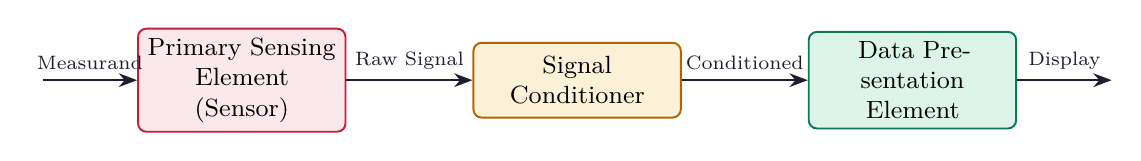
\begin{tikzpicture}[node distance=1.0cm and 1.6cm, thick, font=\small]
  \node[block, fill=hdrred, draw=myred] (sensor) {Primary Sensing\\Element (Sensor)};
  \node[block, right=1.6cm of sensor, fill=hdramber, draw=myamber] (cond) {Signal\\Conditioner};
  \node[block, right=1.6cm of cond, fill=hdrgreen, draw=mygreen] (display) {Data Presentation\\Element};

  % Path lines
  \draw[arrow] ($(sensor.west) - (1.2, 0)$) -- node[above, font=\scriptsize] {Measurand} (sensor.west);
  \draw[arrow] (sensor) -- node[above, font=\scriptsize] {Raw Signal} (cond);
  \draw[arrow] (cond) -- node[above, font=\scriptsize] {Conditioned} (display);
  \draw[arrow] (display.east) -- node[above, font=\scriptsize] {Display} ($(display.east) + (1.2, 0)$);
\end{tikzpicture}
\end{tcolorbox}

% ===============================================================================
\section{Performance Characteristics of Measuring Instruments}
% ===============================================================================

Performance parameters of any measuring device are divided into static and dynamic characteristics.

\subsection{Static Characteristics}
Static characteristics apply when the physical quantity remains constant or changes very slowly.

\begin{tcolorbox}[defbox, title={\textbf{Key Static Characteristics}}]
\begin{itemize}[leftmargin=*, itemsep=3.5pt, topsep=0pt]
  \item \textbf{Accuracy:} The closeness of an instrument reading to the true value of the measurand.
  \item \textbf{Precision:} The degree of reproducibility of measurements (scatter of readings).
  \item \textbf{Resolution:} The smallest change in the input value that can be detected by the instrument.
  \item \textbf{Sensitivity:} The ratio of the change in output deflection ($\Delta \theta_o$) to the change in input physical quantity ($\Delta q_i$): $S = \Delta \theta_o / \Delta q_i$.
  \item \textbf{Repeatability:} The closeness of agreement between successive measurements taken under identical conditions over a short time.
  \item \textbf{Reproducibility:} The consistency of readings taken by different observers, locations, or instruments over a long period.
  \item \textbf{Fidelity:} The ability of a system to reproduce the input signal without dynamic distortion.
  \item \textbf{Static Lag:} The retardation/delay in the response of an instrument to changes in the measurand.
\end{itemize}
\end{tcolorbox}

\subsection{Types of Measurement Errors}
Errors are defined as the difference between the measured value ($A_m$) and the true value ($A_t$). They are classified as:
\begin{enumerate}[label=\alph*., leftmargin=*]
  \item \textbf{Gross Errors:} Caused by human errors in reading, recording, or calculating instruments (e.g., parallax errors).
  \item \textbf{Systematic (Instrumental/Environmental/Observational) Errors:} Errors inherent in the instrument design, environment (temperature, humidity), or calibration drift. These are predictable and can be corrected.
  \item \textbf{Random Errors:} Residual errors that remain after gross and systematic errors have been eliminated. They follow a Gaussian/normal statistical distribution.
\end{enumerate}

\subsection{Dynamic Characteristics}
Dynamic characteristics apply when the input changes rapidly with time. They include:
\begin{itemize}[leftmargin=*, itemsep=2.5pt]
  \item \textbf{Speed of Response:} The rapidity with which the instrument responds to changes in the measurand.
  \item \textbf{Measuring Lag:} Delay in response to a dynamic input.
  \item \textbf{Dynamic Error:} The difference between the true value of a quantity and the value indicated by the instrument under dynamic conditions.
  \item \textbf{Fidelity:} True reproduction of dynamic inputs.
\end{itemize}

% ===============================================================================
\section{Measuring Instruments \& Range Extension}
% ===============================================================================

\subsection{D'Arsonval Movement (PMMC)}
The \textbf{Permanent Magnet Moving Coil (PMMC)} movement is the core analog indicator mechanism. It operates on the electromagnetic force principle: when current flows through a moving coil inside a magnetic field, a deflecting torque is created.
\begin{itemize}[leftmargin=*, itemsep=3.5pt]
  \item \textbf{Deflecting Torque ($T_d$):} $T_d = B \cdot A \cdot N \cdot I$ (where $B$ = flux density, $A$ = coil area, $N$ = turns, $I$ = current).
  \item \textbf{Controlling Torque ($T_c$):} Provided by hair springs: $T_c = K \cdot \theta$ (where $K$ = spring constant, $\theta$ = deflection angle).
  \item \textbf{Balance Condition:} At steady state, $T_d = T_c \implies \theta \propto I$ (linear scale).
  \item \textbf{Drawback:} Measures DC only. AC averages to zero.
\end{itemize}

\subsection{Extension of Range}
PMMC coils are delicate and can handle only small currents (typically $50\,\mu\text{A}$ to $1\,\text{mA}$). For larger ranges, multipliers and shunts are used:

\begin{tcolorbox}[formulabox, title={\textbf{Range Extension Calculations}}]
\begin{enumerate}[leftmargin=*, itemsep=4pt, label=\arabic*.]
  \item \textbf{DC Ammeter Range Extension (Shunt Resistor $R_{sh}$):}
    To measure a total current $I$ using a meter of resistance $R_m$ and full-scale current $I_m$:
    $$I_{sh} \cdot R_{sh} = I_m \cdot R_m \implies (I - I_m)R_{sh} = I_m R_m \implies R_{sh} = \frac{R_m}{\frac{I}{I_m} - 1} = \frac{R_m}{m - 1}$$
    where $m = I/I_m$ is the ammeter multiplying factor.
  \item \textbf{DC Voltmeter Range Extension (Multiplier Resistor $R_s$):}
    To measure a total voltage $V$ using a meter of resistance $R_m$ and full-scale voltage $V_m = I_m R_m$:
    $$V = I_m (R_s + R_m) \implies R_s + R_m = \frac{V}{I_m} \implies R_s = R_m \left(\frac{V}{V_m} - 1\right) = R_m(m - 1)$$
    where $m = V/V_m$ is the voltmeter multiplying factor.
\end{enumerate}
\end{tcolorbox}

\subsection{True RMS Responding Voltmeter}
Standard AC meters measure the average value and scale it by $1.11$ to indicate RMS for perfect sine waves. For non-sinusoidal waves, this causes massive errors.

\begin{itemize}[leftmargin=*, itemsep=3.5pt]
  \item \textbf{Working Principle:} True RMS voltmeters use a \textbf{thermocouple/heating element} combination. The input AC voltage is fed into a heater resistor, producing heat proportional to the RMS power ($\text{Heat} \propto V_{\text{rms}}^2$). A thermocouple converts the temperature difference into a DC voltage, driving a standard PMMC meter to indicate the true RMS value of any waveform.
\end{itemize}

% ===============================================================================
\section{Ohmmeters}
% ===============================================================================

\begin{tcolorbox}[defbox, title={\textbf{Ohmmeter}}]
An \textbf{ohmmeter} is an instrument designed to measure electrical resistance. It consists of an internal voltage source (battery), a current-limiting resistor, and a current-sensing movement (typically PMMC) that displays the resistance value on a calibrated scale.
\end{tcolorbox}

Ohmmeters are classified into two primary designs depending on how the unknown resistor $R_x$ is connected to the meter: \textbf{Series-type} and \textbf{Shunt-type}.

\subsection{Series-Type Ohmmeter}
A series-type ohmmeter connects the unknown resistor $R_x$ in series with the internal circuit. It is primarily used for measuring high resistance values (typically in the range of kilohms to megohms).

\begin{itemize}[leftmargin=*, itemsep=3.5pt]
  \item \textbf{Circuit Operation:}
    \begin{itemize}[leftmargin=*, itemsep=2.5pt, topsep=0pt]
      \item $E$: Internal battery voltage source.
      \item $R_1$: Series current-limiting resistor to protect the meter.
      \item $R_2$: Shunt zero-adjust variable resistor across the PMMC meter.
      \item $R_m$: Internal resistance of the PMMC movement.
      \item $A, B$: Connection terminals for the unknown resistor $R_x$.
    \end{itemize}
  \item \textbf{Calibration \& Zero Adjustment:}
    \begin{itemize}[leftmargin=*, itemsep=2.5pt, topsep=0pt]
      \item \textbf{Short Circuit ($R_x = 0$):} Terminals A and B are short-circuited. The total current is maximum, and the shunt resistor $R_2$ is adjusted so that the pointer deflects to its full-scale value. This Full Scale Deflection (FSD) point is marked as $0\,\Omega$ on the right side of the scale.
      \item \textbf{Open Circuit ($R_x = \infty$):} Terminals A and B are left open. The current is zero. The pointer remains at zero deflection, which is marked as $\infty\,\Omega$ on the left side of the scale.
    \end{itemize}
  \item \textbf{Scale Characteristic:} The scale is non-linear and runs from right to left ($0\,\Omega$ at FSD on the right, $\infty\,\Omega$ at zero deflection on the left). It is crowded at the high-resistance end (left).
\end{itemize}

\begin{tcolorbox}[tikzbox, title={Series-Type Ohmmeter Circuit Schematic}]
\centering
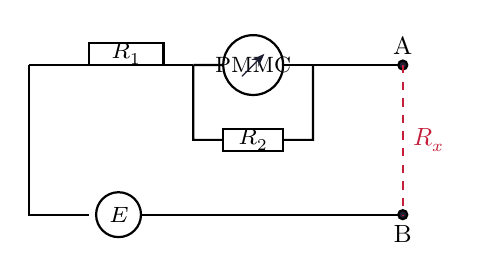
\begin{tikzpicture}[thick, scale=0.95]
  % Coordinates
  \coordinate (start) at (0,2);
  \coordinate (R1_in) at (0.8,2);
  \coordinate (R1_out) at (1.8,2);
  \coordinate (node_shunt_left) at (2.2,2);
  \coordinate (node_shunt_right) at (3.8,2);
  \coordinate (M_in) at (2.6,2);
  \coordinate (M_out) at (3.4,2);
  \coordinate (A_term) at (5.0,2);
  \coordinate (B_term) at (5.0,0);
  \coordinate (E_in) at (0,0);
  \coordinate (E_out) at (0.8,0);

  % Draw main loop
  \draw (start) -- (R1_in);
  \draw[fill=white] (R1_in) rectangle (1.8,2.3) node[midway] {\footnotesize $R_1$};
  \draw (R1_out) -- (node_shunt_left);
  \draw (node_shunt_left) -- (2.6,2);
  
  % PMMC Meter
  \draw[fill=white] (3.0,2) circle (0.4) node (M) {\footnotesize PMMC};
  \draw[arrow, thin] (2.85,1.85) -- (3.15,2.15);
  \draw (2.6,2) -- (M_in);
  \draw (M_out) -- (node_shunt_right);
  \draw (node_shunt_right) -- (A_term);
  
  % Shunt R2 path
  \draw (node_shunt_left) -- (2.2,1.0) -- (2.6,1.0);
  \draw[fill=white] (2.6,0.85) rectangle (3.4,1.15) node[midway] {\footnotesize $R_2$};
  \draw (3.4,1.0) -- (3.8,1.0) -- (node_shunt_right);
  
  % Bottom wire and Battery
  \draw (start) -- (0,0) -- (0.8,0);
  \draw[fill=white] (1.2, 0) circle (0.3) node {\footnotesize $E$};
  \draw (1.5,0) -- (B_term);
  
  % Terminals
  \draw[fill=mydark] (A_term) circle (0.06) node[above] {\small A};
  \draw[fill=mydark] (B_term) circle (0.06) node[below] {\small B};
  
  % Unknown Rx
  \draw[dashed, myred, thick] (A_term) -- (B_term) node[midway, right] {\small $R_x$};
\end{tikzpicture}
\end{tcolorbox}

\begin{tcolorbox}[formulabox, title={\textbf{Series Ohmmeter Equations}}]
The meter current $I_m$ as a function of the unknown resistance $R_x$ is:
\begin{equation}
  I_m = \frac{E \cdot R_2}{(R_x + R_1)(R_2 + R_m) + R_2 R_m}
\end{equation}
Let $R_h$ be the half-scale resistance (the value of $R_x$ when $I_m = 0.5 I_{fs}$):
\begin{equation}
  R_h = R_1 + \frac{R_2 R_m}{R_2 + R_m}
\end{equation}
The deflection ratio $s = I_m / I_{fs}$ is given by:
\begin{equation}
  s = \frac{R_h}{R_x + R_h}
\end{equation}
\end{tcolorbox}

\subsection{Shunt-Type Ohmmeter}
A shunt-type ohmmeter connects the unknown resistor $R_x$ in parallel (shunt) with the PMMC meter. It is primarily used for measuring very low resistance values (typically $1\,\Omega$ to $100\,\Omega$).

\begin{itemize}[leftmargin=*, itemsep=3.5pt]
  \item \textbf{Circuit Operation:}
    \begin{itemize}[leftmargin=*, itemsep=2.5pt, topsep=0pt]
      \item $E$: Internal battery voltage source.
      \item $R_1$: Series adjustable current-limiting resistor to calibrate the meter and limit battery drain.
      \item $S$: Switch to disconnect the battery when not in use.
      \item $R_m$: Internal resistance of the PMMC movement.
      \item $A, B$: Connection terminals for $R_x$ across the meter.
    \end{itemize}
  \item \textbf{Calibration \& Zero Adjustment:}
    \begin{itemize}[leftmargin=*, itemsep=2.5pt, topsep=0pt]
      \item \textbf{Short Circuit ($R_x = 0$):} Terminals A and B are short-circuited. No current flows through the meter ($I_m = 0$). The pointer remains at zero deflection on the left, which is marked as $0\,\Omega$.
      \item \textbf{Open Circuit ($R_x = \infty$):} Terminals A and B are open-circuited. All current flows through the meter. $R_1$ is adjusted until the meter deflects to FSD, which is marked as $\infty\,\Omega$ on the right side of the scale.
    \end{itemize}
  \item \textbf{Scale Characteristic:} The scale is non-linear and runs from left to right ($0\,\Omega$ at zero deflection on the left, $\infty\,\Omega$ at FSD on the right). It is suitable for low-value resistance measurement since low values cause measurable deflection changes near zero.
\end{itemize}

\begin{tcolorbox}[tikzbox, title={Shunt-Type Ohmmeter Circuit Schematic}]
\centering
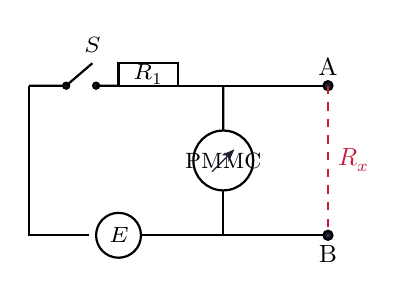
\begin{tikzpicture}[thick, scale=0.95]
  % Coordinates
  \coordinate (start) at (0,2);
  \coordinate (R1_in) at (1.2,2);
  \coordinate (R1_out) at (2.0,2);
  \coordinate (node_meter) at (2.6,2);
  \coordinate (node_term_A) at (4.0,2);
  \coordinate (E_in) at (0,0);
  \coordinate (B_term) at (4.0,0);
  
  % Draw top path with Switch
  \draw (start) -- (0.5,2);
  \draw[fill=mydark] (0.5,2) circle (0.04);
  \draw[fill=mydark] (0.9,2) circle (0.04);
  \draw (0.5,2) -- (0.85,2.3) node[above] {\footnotesize $S$};
  \draw (0.9,2) -- (R1_in);
  \draw[fill=white] (R1_in) rectangle (2.0,2.3) node[midway] {\footnotesize $R_1$};
  \draw (R1_out) -- (node_meter);
  \draw (node_meter) -- (node_term_A);
  
  % PMMC Meter branch
  \draw (node_meter) -- (2.6,1.4);
  \draw[fill=white] (2.6,1.0) circle (0.4) node {\footnotesize PMMC};
  \draw[arrow, thin] (2.45,0.85) -- (2.75,1.15);
  \draw (2.6,0.6) -- (2.6,0);
  
  % Battery
  \draw (start) -- (0,0) -- (0.8,0);
  \draw[fill=white] (1.2, 0) circle (0.3) node {\footnotesize $E$};
  \draw (1.5,0) -- (B_term);
  
  % Connections at bottom
  \draw (2.6,0) -- (B_term);
  
  % Terminals
  \draw[fill=mydark] (node_term_A) circle (0.06) node[above] {\small A};
  \draw[fill=mydark] (B_term) circle (0.06) node[below] {\small B};
  
  % Unknown Rx
  \draw[dashed, myred, thick] (node_term_A) -- (B_term) node[midway, right] {\small $R_x$};
\end{tikzpicture}
\end{tcolorbox}

\begin{tcolorbox}[formulabox, title={\textbf{Shunt Ohmmeter Equations}}]
The meter current $I_m$ is given by:
\begin{equation}
  I_m = \frac{E R_x}{R_1(R_x + R_m) + R_x R_m}
\end{equation}
When $R_1 \gg R_m$, we can simplify to:
\begin{equation}
  I_m \approx \frac{E}{R_1} \left( \frac{R_x}{R_x + R_m} \right)
\end{equation}
The half-scale resistance $R_h$ where $I_m = 0.5 I_{fs}$ is approximately:
\begin{equation}
  R_h = \frac{R_1 R_m}{R_1 + R_m} \approx R_m
\end{equation}
The deflection ratio $s = I_m / I_{fs}$ is:
\begin{equation}
  s = \frac{R_x}{R_x + R_h}
\end{equation}
\end{tcolorbox}

% ===============================================================================
\section{Multimeters}
% ===============================================================================

\begin{tcolorbox}[defbox, title={\textbf{Multimeter}}]
A \textbf{multimeter} is a multi-purpose electronic measuring instrument that integrates several measurement functions---typically voltage, current, and resistance---into a single device.
\end{tcolorbox}

Multimeters are available in two forms: \textbf{Analog Multimeters} (often called VOM) and \textbf{Digital Multimeters} (DMM).

\subsection{Analog Multimeter (VOM)}
An Analog Multimeter (Volt-Ohm-Milliammeter or VOM) uses a standard PMMC movement as the central indicator. A multi-deck, multi-position rotary selector switch connects different internal networks to the meter.

\begin{itemize}[leftmargin=*, itemsep=3.5pt]
  \item \textbf{Sub-circuits \& Function Selection:}
    \begin{itemize}[leftmargin=*, itemsep=2.5pt, topsep=0pt]
      \item \textbf{DC Voltage:} Extends range using series multiplier resistors.
      \item \textbf{AC Voltage:} Uses a diode rectifier network (half-wave or full-wave) to convert AC to DC, which is then scaled by series multipliers.
      \item \textbf{DC Current:} Extends range using parallel shunt resistors.
      \item \textbf{Resistance:} Uses an internal battery and calibrating resistors configured as series or shunt ohmmeters.
    \end{itemize}
  \item \textbf{Sensitivity:} Voltmeter sensitivity is expressed in ohms-per-volt ($\Omega/\text{V}$), equal to $1 / I_{fs}$. A typical VOM has a DC sensitivity of $20\,\text{k}\Omega/\text{V}$.
\end{itemize}

\begin{tcolorbox}[tikzbox, title={Analog Multimeter (VOM) Block Schematic}]
\centering
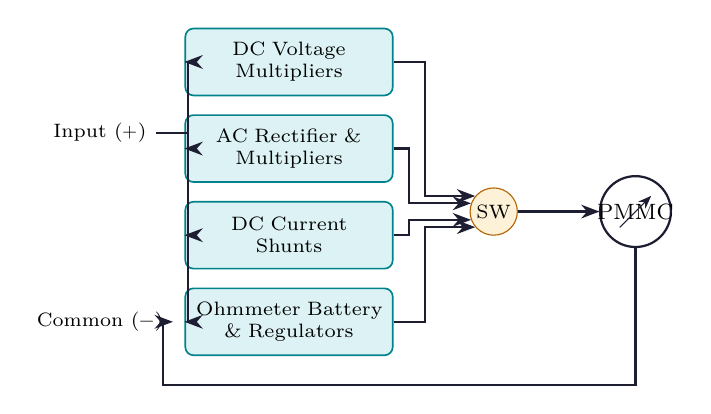
\begin{tikzpicture}[font=\small, >=Stealth,
  sblock/.style={rectangle, draw=myteal, fill=hdrteal, text width=2.4cm,
    align=center, minimum height=0.85cm, font=\scriptsize,
    rounded corners=3pt, line width=0.6pt}]
  
  % Input terminals on left
  \node (input) at (0, 1.8) {\scriptsize Input ($+$)};
  \node (common) at (0, -0.6) {\scriptsize Common ($-$)};

  % Blocks positioned with clear vertical separation
  \node[sblock] (dcv) at (2.4, 2.7) {DC Voltage\\Multipliers};
  \node[sblock] (acv) at (2.4, 1.6) {AC Rectifier \&\\Multipliers};
  \node[sblock] (dci) at (2.4, 0.5) {DC Current\\Shunts};
  \node[sblock] (ohm) at (2.4, -0.6) {Ohmmeter Battery\\\& Regulators};

  % Selector Switch
  \node[circle, draw=myamber, fill=hdramber, minimum size=0.6cm, inner sep=0pt] (sw) at (5.0, 0.8) {\scriptsize SW};

  % PMMC Meter
  \node[circle, draw=mydark, fill=white, minimum size=0.9cm] (pmmc) at (6.8, 0.8) {};
  \draw[thick, color=mydark] (pmmc.center) circle (0.45);
  \node at (pmmc.center) {\footnotesize PMMC};
  \draw[arrow, thin] ($(pmmc.center)+(-0.2,-0.2)$) -- ($(pmmc.center)+(0.2,0.2)$);

  % Connections from Input to Blocks
  \draw[arrow] (input.east) -- ++(0.4, 0) |- (dcv.west);
  \draw[arrow] (input.east) -- ++(0.4, 0) |- (acv.west);
  \draw[arrow] (input.east) -- ++(0.4, 0) |- (dci.west);
  \draw[arrow] (input.east) -- ++(0.4, 0) |- (ohm.west);

  % Connections from Blocks to Selector Switch (SW)
  \draw[arrow] (dcv.east) -- ++(0.4, 0) |- (sw.140);
  \draw[arrow] (acv.east) -- ++(0.2, 0) |- (sw.160);
  \draw[arrow] (dci.east) -- ++(0.2, 0) |- (sw.200);
  \draw[arrow] (ohm.east) -- ++(0.4, 0) |- (sw.220);

  % Switch to PMMC
  \draw[arrow] (sw.east) -- (pmmc.west);

  % PMMC Return to Common (completely clear of all blocks, going below the bottom block)
  \draw[arrow] (pmmc.south) -- (6.8, -1.4) -- (0.8, -1.4) |- (common.east);
\end{tikzpicture}
\end{tcolorbox}

\subsection{Digital Multimeter (DMM)}
A Digital Multimeter (DMM) processes signals electronically and displays the measured values numerically. DMMs offer higher accuracy, higher input impedance ($10\,\text{M}\Omega$ to eliminate loading effects), and auto-ranging capabilities.

\begin{itemize}[leftmargin=*, itemsep=3.5pt]
  \item \textbf{Signal Conditioning Stages:}
    \begin{itemize}[leftmargin=*, itemsep=2.5pt, topsep=0pt]
      \item \textbf{AC Voltage:} Scale down by an attenuator and convert to DC using an active precision rectifier.
      \item \textbf{DC Current:} Force the current through low-resistance shunts and measure the resulting voltage drop.
      \item \textbf{Resistance:} Pass a constant current from an internal source through the unknown resistor $R_x$ to generate a voltage drop ($V_x = I_{\text{const}} \cdot R_x$).
    \end{itemize}
  \item \textbf{Dual-Slope Integration ADC:} DMMs use a Dual-Slope ADC for converting analog voltages into digital form due to its superior noise rejection.
\end{itemize}

\begin{tcolorbox}[tikzbox, title={Digital Multimeter (DMM) Block Diagram}]
\centering
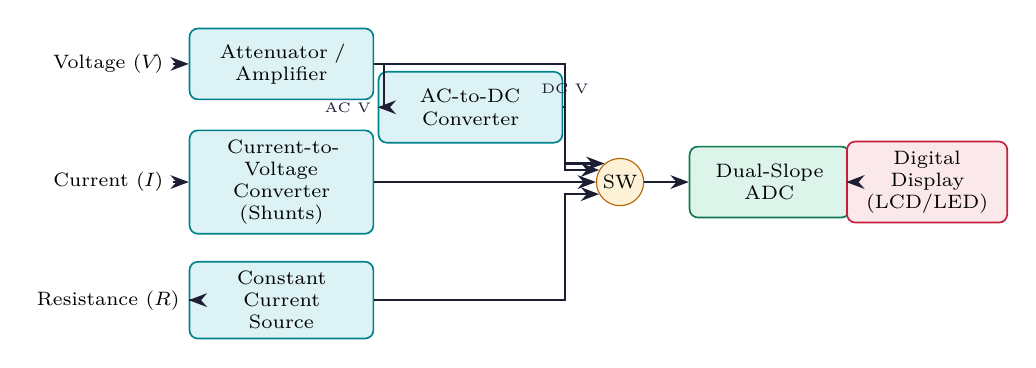
\begin{tikzpicture}[font=\small, >=Stealth,
  sblock/.style={rectangle, draw=myteal, fill=hdrteal, text width=2.1cm,
    align=center, minimum height=0.9cm, font=\scriptsize,
    rounded corners=3pt, line width=0.6pt}]
  
  % Inputs on the left
  \node (in_v) at (0, 2.4) {\scriptsize Voltage ($V$)};
  \node (in_i) at (0, 0.9) {\scriptsize Current ($I$)};
  \node (in_r) at (0, -0.6) {\scriptsize Resistance ($R$)};
  
  % First-stage blocks
  \node[sblock] (attn) at (2.2, 2.4) {Attenuator /\\Amplifier};
  \node[sblock] (shunt) at (2.2, 0.9) {Current-to-Voltage\\Converter (Shunts)};
  \node[sblock] (const_i) at (2.2, -0.6) {Constant Current\\Source};
  
  % AC-to-DC Converter (lowered for clear branching)
  \node[sblock] (rect) at (4.6, 1.85) {AC-to-DC\\Converter};
  
  % Selector Switch (SW)
  \node[circle, draw=myamber, fill=hdramber, minimum size=0.6cm, inner sep=0pt] (sw) at (6.5, 0.9) {\scriptsize SW};
  
  % ADC & Display
  \node[sblock, fill=hdrgreen, draw=mygreen, text width=1.8cm] (adc) at (8.4, 0.9) {Dual-Slope\\ADC};
  \node[sblock, fill=hdrred, draw=myred, text width=1.8cm] (disp) at (10.4, 0.9) {Digital Display\\(LCD/LED)};
  
  % Connections
  % Voltage path
  \draw[arrow] (in_v) -- (attn);
  \draw[line] (attn.east) -- (3.5, 2.4) coordinate (v_split);
  \draw[arrow] (v_split) -- (5.8, 2.4) |- (sw.130) node[pos=0.2, above, font=\tiny] {DC V};
  \draw[arrow] (v_split) |- (rect.west) node[pos=0.7, left, font=\tiny] {AC V};
  \draw[arrow] (rect.east) -- (5.8, 1.85) |- (sw.150);
  
  % Current path
  \draw[arrow] (in_i) -- (shunt);
  \draw[arrow] (shunt.east) -- (sw.180);
  
  % Resistance path
  \draw[arrow] (in_r) -- (const_i);
  \draw[arrow] (const_i.east) -- (5.8, -0.6) |- (sw.210);
  
  % Switch to ADC and Display
  \draw[arrow] (sw.east) -- (adc.west);
  \draw[arrow] (adc.east) -- (disp.west);
\end{tikzpicture}
\tcbset{breakable}
\end{tcolorbox}

\begin{tcolorbox}[formulabox, title={\textbf{Dual-Slope ADC Integration Principle}}]
The Dual-Slope ADC operates in two phases:
\begin{enumerate}[leftmargin=*, itemsep=2.5pt]
  \item \textbf{Integrate Phase (Fixed Time $T_1$):} The input voltage $V_{\text{in}}$ is integrated for a predetermined fixed duration $T_1 = 2^N \cdot T_{\text{clk}}$. The integrator output voltage rises to:
    \begin{equation}
      V_p = -\frac{V_{\text{in}}}{RC} T_1
    \end{equation}
  \item \textbf{De-integrate Phase (Variable Time $T_2$):} A reference voltage $-V_{\text{ref}}$ of opposite polarity is connected to the integrator. The output ramps down to zero at a constant rate. The variable time $T_2$ taken to return to zero is measured by counting clock pulses:
    \begin{equation}
      V_p = \frac{V_{\text{ref}}}{RC} T_2
    \end{equation}
\end{enumerate}
Equating the two peak values, we obtain the voltage relationship:
\begin{equation}
  V_{\text{in}} = V_{\text{ref}} \left( \frac{T_2}{T_1} \right)
\end{equation}
\textbf{Key Advantage:} The measurement depends only on the ratio of times $T_2/T_1$ and $V_{\text{ref}}$, completely eliminating errors due to component tolerances/aging of $R$ and $C$ or clock frequency drift.
\end{tcolorbox}

\newpage
% ===============================================================================
% MANDATORY QUICK REVISION PAGE
% ===============================================================================
\begin{center}
  {\large\bfseries\color{myred} Quick Revision --- Module 1}\\[3pt]
  {\small\color{mydark} Block Schematics \& Basic Instruments $|$ OE-EC604A}
\end{center}
\noindent{\color{myred}\rule{\linewidth}{1.2pt}}
\vspace{4pt}

\begin{tcolorbox}[formulabox, title={\textbf{Key Formulas at a Glance}}]
\begin{align*}
  \text{Ammeter Shunt:} \quad & R_{sh} = \frac{R_m}{m - 1} \quad \text{where} \ m = \frac{I}{I_m} \\
  \text{Voltmeter Multiplier:} \quad & R_s = R_m(m - 1) \quad \text{where} \ m = \frac{V}{V_m} \\
  \text{Series Ohmmeter Deflection:} \quad & s = \frac{I_m}{I_{fs}} = \frac{R_h}{R_x + R_h} \quad \text{where} \ R_h = R_1 + R_2 \parallel R_m \\
  \text{Shunt Ohmmeter Deflection:} \quad & s = \frac{I_m}{I_{fs}} = \frac{R_x}{R_x + R_h} \quad \text{where} \ R_h = R_1 \parallel R_m \approx R_m \\
  \text{DMM Dual-Slope ADC:} \quad & V_{\text{in}} = V_{\text{ref}} \left(\frac{T_2}{T_1}\right)
\end{align*}
\end{tcolorbox}

\begin{tcolorbox}[defbox, title={\textbf{One-Line Definitions}}]
\begin{itemize}[leftmargin=*, itemsep=2.5pt, topsep=0pt]
  \item \textbf{Accuracy:} Degree of closeness of a measured value to the actual true value.
  \item \textbf{Precision:} Degree of agreement/repeatability within a group of measurements.
  \item \textbf{Resolution:} The smallest detectable change in the input measurand.
  \item \textbf{PMMC:} Permanent Magnet Moving Coil movement; sensitive DC indicator based on magnetic coil torque.
  \item \textbf{True RMS Voltmeter:} Instrument measuring heating power of input signal to compute exact RMS regardless of shape.
  \item \textbf{Series-type Ohmmeter:} Ohmmeter where the unknown resistance is in series with the meter; zero is on the right of the scale.
  \item \textbf{Shunt-type Ohmmeter:} Ohmmeter where the unknown resistance is in parallel with the meter; zero is on the left of the scale.
  \item \textbf{Dual-Slope ADC:} An analog-to-digital converter that integrates input voltage and then de-integrates reference voltage, rejecting noise.
\end{itemize}
\end{tcolorbox}

\begin{tcolorbox}[exambox, title={\textbf{Frequently Asked / Viva Questions}}]
\begin{enumerate}[topsep=0pt, label=\textbf{Q\arabic*.}, itemsep=5pt]
  \item \Q{Differentiate between Accuracy and Precision.}
    Accuracy is the closeness of a measured value to the true value, whereas precision is the repeatability of readings when measured repeatedly. An instrument can be highly precise but inaccurate if it has a constant offset error.
  \item \Q{A PMMC meter has internal resistance $R_m = 100\,\Omega$ and full-scale deflection current $I_m = 1\,\text{mA}$. Calculate the shunt resistance required to extend its range to $1\,\text{A}$.}\\
    Given: $R_m = 100\,\Omega$, $I_m = 1\,\text{mA} = 0.001\,\text{A}$, Target current $I = 1\,\text{A}$.\par
    Multiplying factor: $m = I / I_m = 1 / 0.001 = 1000$.\par
    Shunt resistance: $R_{sh} = R_m / (m - 1) = 100 / (1000 - 1) = 100 / 999 \approx 0.1001\,\Omega$.
  \item \Q{Using the same PMMC meter ($R_m=100\,\Omega, I_m=1\,\text{mA}$), calculate the multiplier resistance required to extend its range to measure a voltmeter scale of $100\,\text{V}$.}\\
    Full scale meter voltage: $V_m = I_m \cdot R_m = 0.001 \times 100 = 0.1\,\text{V}$.\par
    Multiplying factor: $m = V / V_m = 100 / 0.1 = 1000$.\par
    Multiplier series resistance: $R_s = R_m(m - 1) = 100 \times 999 = 99,900\,\Omega = 99.9\,\text{k}\Omega$.
  \item \Q{Why does a PMMC instrument fail to measure AC values directly?}
    Because the direction of deflecting torque depends on the current polarity. For AC, the current alternates polarity rapidly (e.g., $50\,\text{Hz}$). The pointer attempts to follow the oscillations but due to inertia, it stays at zero, displaying only the average value (which is 0 for AC).
  \item \Q{What is True RMS and why is it preferred over average-responding voltmeters?}
    Average-responding voltmeters rectify AC, find the average, and multiply it by $1.11$ (the form factor for a sine wave) to display RMS. This is invalid for square, triangular, or distorted waves. A True RMS voltmeter measures the actual thermal power generated by the signal, representing its true heating equivalent.
  \item \Q{Compare Series and Shunt type Ohmmeters.}
    In a series ohmmeter, the unknown resistor $R_x$ is in series with the PMMC meter. Zero resistance ($0\,\Omega$) corresponds to full-scale deflection (FSD) on the right. In a shunt ohmmeter, $R_x$ is in parallel with the meter. Zero resistance ($0\,\Omega$) corresponds to zero deflection on the left.
  \item \Q{What is the main advantage of a Digital Multimeter (DMM) over an analog VOM?}
    A DMM provides high input impedance (typically $10\,\text{M}\Omega$ across all ranges), which prevents loading errors. It also offers digital numerical displays (no parallax errors), auto-ranging, and greater accuracy.
  \item \Q{Explain why a Dual-Slope ADC is preferred in DMMs.}
    It has excellent noise rejection (particularly line frequency noise like $50\,\text{Hz}$/ $60\,\text{Hz}$ if integration time is chosen as a multiple of the line period). Additionally, the conversion accuracy is independent of the values of the integrating capacitor and resistor, and the clock frequency.
  \item \Q{What are systematic errors and how can they be minimized?}
    Systematic errors are predictable, constant errors arising from instrument calibration, component aging, or environmental changes (temperature/humidity). They can be minimized by periodic calibration, proper shielding, and applying mathematical correction factors.
  \item \Q{What is static lag and how does it differ from dynamic lag?}
    Static lag is the delay in response when the input measurand is constant or changing very slowly, caused by friction or spring inertia. Dynamic lag occurs when the input changes rapidly, caused by the system's dynamic parameters (mass, damping, capacitance).
\end{enumerate}
\end{tcolorbox}

\begin{tcolorbox}[tikzbox, title={Accuracy vs Precision Comparison Summary}]
\renewcommand{\arraystretch}{1.4}
\par\noindent
\begin{tabularx}{\linewidth}{|B{2.2cm}|>{\small\centering\arraybackslash}X|>{\small\centering\arraybackslash}X|}
\hline
\textbf{Feature} & \textbf{\color{myred}Accuracy} & \textbf{\color{myteal}Precision} \\
\hline
\textbf{Core Concept} & Closeness to the actual true value. & Closeness of multiple readings to each other. \\
\hline
\textbf{Error Type} & Linked to systematic errors. & Linked to random errors (scatter). \\
\hline
\textbf{Calibration} & Can be improved by calibration. & Calibration does not improve precision. \\
\hline
\textbf{Dependence} & Requires precision to be accurate. & Can be highly precise but inaccurate. \\
\hline
\textbf{Time Period} & Measured over short term. & Represents stability over short term. \\
\hline
\end{tabularx}
\end{tcolorbox}



% -- Module 2 -----------------------------------------------------------------
\modulestart{2}{Signal Analyzers}

\section{Signal Analyzers}
% ===============================================================================

Signal analyzers resolve electrical signals into their individual frequency components, measuring amplitude, distortion, and spectral properties.

\subsection{Wave Analyzers}
A \textbf{Wave Analyzer} is an instrument designed to measure the amplitude of a single frequency component of a complex signal.
\begin{itemize}[leftmargin=*, itemsep=3pt]
  \item \textbf{AF Wave Analyzer:} Uses a frequency-selective amplifier with a tunable active filter (Wein bridge or RC network) to isolate the target frequency.
  \item \textbf{Heterodyne Wave Analyzer (HF):} Operates on the superheterodyne principle. The input signal is up-converted to a high Intermediate Frequency (IF) using a tunable Local Oscillator and Mixer. A narrow-band bandpass filter extracts the target frequency, which is then rectified and indicated on a PMMC meter.
\end{itemize}

\begin{tcolorbox}[tikzbox, title={Heterodyne Wave Analyzer Block Diagram}]
\centering
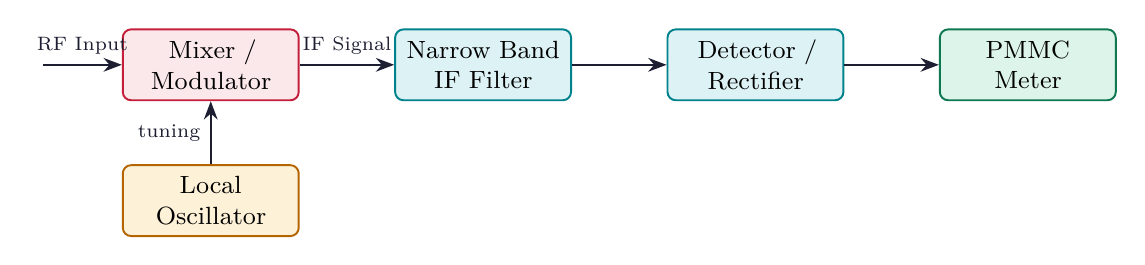
\begin{tikzpicture}[node distance=0.6cm and 1.2cm, thick, font=\small,
  sblock/.style={rectangle, draw=myteal, fill=hdrteal, text width=2.0cm,
    align=center, minimum height=0.9cm, font=\small, rounded corners=3pt, line width=0.7pt},
  sred/.style={rectangle, draw=myred, fill=hdrred, text width=2.0cm,
    align=center, minimum height=0.9cm, font=\small, rounded corners=3pt, line width=0.7pt},
  samber/.style={rectangle, draw=myamber, fill=hdramber, text width=2.0cm,
    align=center, minimum height=0.9cm, font=\small, rounded corners=3pt, line width=0.7pt},
  sgreen/.style={rectangle, draw=mygreen, fill=hdrgreen, text width=2.0cm,
    align=center, minimum height=0.9cm, font=\small, rounded corners=3pt, line width=0.7pt}]

  \node[sred] (mixer) {Mixer /\\Modulator};
  \node[sblock, right=of mixer] (filter) {Narrow Band\\IF Filter};
  \node[sblock, right=of filter] (det) {Detector /\\Rectifier};
  \node[sgreen, right=of det] (meter) {PMMC\\Meter};
  \node[samber, below=0.8cm of mixer] (lo) {Local\\Oscillator};

  % Paths
  \draw[arrow] ($(mixer.west) - (1.0, 0)$) -- node[above, font=\scriptsize] {RF Input} (mixer.west);
  \draw[arrow] (mixer) -- node[above, font=\scriptsize] {IF Signal} (filter);
  \draw[arrow] (filter) -- (det);
  \draw[arrow] (det) -- (meter);
  \draw[arrow] (lo) -- node[left, font=\scriptsize] {tuning} (mixer);
\end{tikzpicture}
\tcbset{breakable}
\end{tcolorbox}

\subsection{Total Harmonic Distortion (THD)}
Distortion analyzers measure the deviation of a waveform from a perfect sinusoid. When a pure sine wave passes through a non-linear device, harmonics are generated.

\begin{tcolorbox}[formulabox, title={\textbf{Harmonic Distortion Calculations}}]
Let $V_1$ be the fundamental component amplitude, and $V_2, V_3, \dots, V_n$ be the amplitudes of the second, third, and higher order harmonics.
\begin{itemize}[leftmargin=*, itemsep=3.5pt, topsep=0pt]
  \item \textbf{Individual Harmonic Distortion ($D_n$):}
    $$D_n = \frac{V_n}{V_1} \times 100\%$$
  \item \textbf{Total Harmonic Distortion (THD):}
    $$\text{THD} = \frac{\sqrt{V_2^2 + V_3^2 + V_4^2 + \dots + V_n^2}}{V_1}$$
  \item \textbf{THD relative to Total RMS Value ($V_{\text{rms}}$):}
    $$\text{THD}_t = \frac{\sqrt{V_2^2 + V_3^2 + \dots + V_n^2}}{\sqrt{V_1^2 + V_2^2 + \dots + V_n^2}} = \frac{\sqrt{V_{\text{rms}}^2 - V_1^2}}{V_{\text{rms}}}$$
\end{itemize}
\end{tcolorbox}

\subsection{Spectrum Analyzers}
Unlike wave analyzers that measure one frequency component at a time, a \textbf{Spectrum Analyzer} swept-tunes across a frequency band and displays the entire frequency spectrum (amplitude vs frequency) on a screen.
- \textbf{Working:} A saw-tooth sweep generator sweeps the tuning voltage of a Voltage Controlled Oscillator (VCO). This VCO serves as the local oscillator for a superheterodyne mixer, sweeping the input signal past a narrow bandpass filter. The output is rectified and drives the vertical deflection of a CRT, while the saw-tooth generator drives the horizontal sweep, yielding the spectral display.

% ===============================================================================
\section{Signal Generators}
% ===============================================================================

Signal generators produce controlled electrical waveforms for testing, calibration, and troubleshooting.

\subsection{Function Generators}
A \textbf{Function Generator} produces multiple standard waveforms (sine, square, triangular) over a wide frequency range.
- \textbf{Working Principle:} It utilizes an \textbf{integrator} and a \textbf{comparator (Schmitt trigger)} feed-back loop. The integrator charges/discharges a capacitor using constant current sources, yielding a linear triangular wave. The comparator toggles its output state at peak voltages, yielding a square wave. The triangular wave is fed through a diode-resistance wave-shaping network to approximate a low-distortion sine wave.

\subsection{Arbitrary Waveform Generators (AWG)}
An \textbf{AWG} generates custom, user-defined waveforms. It functions digitally:
1. The user defines the waveform shape mathematically or via sampling, storing the digital coordinates in a \textbf{Waveform Memory}.
2. A \textbf{Sampling Clock} drives an address counter to read out the digital words sequentially.
3. A high-speed \textbf{Digital-to-Analog Converter (DAC)} converts the digital words back into a continuous analog voltage.
4. A \textbf{Reconstruction Filter} smooths out the quantization steps.

\newpage
% ===============================================================================
% MANDATORY QUICK REVISION PAGE
% ===============================================================================
\begin{center}
  {\large\bfseries\color{myred} Quick Revision --- Module 2}\\[3pt]
  {\small\color{mydark} Signal Analyzers \& Generators $|$ OE-EC604A}
\end{center}
\noindent{\color{myred}\rule{\linewidth}{1.2pt}}
\vspace{4pt}

\begin{tcolorbox}[formulabox, title={\textbf{Key Distortion Formula}}]
$$\text{THD} = \frac{\sqrt{V_2^2 + V_3^2 + \dots + V_n^2}}{V_1} \qquad D_n = \frac{V_n}{V_1}$$
$$\text{Total AC Power RMS:} \quad V_{\text{rms}} = \sqrt{V_1^2 + V_2^2 + V_3^2 + \dots}$$
\end{tcolorbox}

\begin{tcolorbox}[defbox, title={\textbf{One-Line Definitions}}]
\begin{itemize}[leftmargin=*, itemsep=2.5pt, topsep=0pt]
  \item \textbf{Wave Analyzer:} Frequency-selective voltmeter tuned to measure a single harmonic component.
  \item \textbf{Spectrum Analyzer:} Swept-frequency instrument displaying amplitude vs frequency across a band.
  \item \textbf{THD:} Total Harmonic Distortion; ratio of root-sum-square of all harmonics to fundamental amplitude.
  \item \textbf{Function Generator:} Signal source using integrator-comparator loops to yield sine, square, and triangle waves.
  \item \textbf{Sweep Generator:} Generator sweeping output frequency automatically across a range for response plotting.
  \item \textbf{AWG:} Arbitrary Waveform Generator; digitally synthesises arbitrary user-defined waveforms from RAM.
\end{itemize}
\end{tcolorbox}

\begin{tcolorbox}[exambox, title={\textbf{Frequently Asked / Viva Questions}}]
\begin{enumerate}[topsep=0pt, label=\textbf{Q\arabic*.}, itemsep=5pt]
  \item \Q{Compare Wave Analyzers and Spectrum Analyzers.}
    A wave analyzer is a narrow-band selective voltmeter tuned manually to measure a single isolated frequency component. A spectrum analyzer automatically sweeps across a band of frequencies and displays the entire spectrum (amplitude vs frequency) in real-time.
  \item \Q{An instrument measures a fundamental component $V_1 = 10\,\text{V}$ and harmonics $V_2 = 1\,\text{V}$, $V_3 = 0.5\,\text{V}$. Calculate the THD.}\\
    Harmonic RMS: $V_h = \sqrt{V_2^2 + V_3^2} = \sqrt{1^2 + 0.5^2} = \sqrt{1 + 0.25} = \sqrt{1.25} \approx 1.118\,\text{V}$.\par
    $\text{THD} = V_h / V_1 = 1.118 / 10 = 0.1118 \implies 11.18\%$.
  \item \Q{Explain the working principle of a basic Function Generator.}
    A function generator uses an integrator and a Schmitt trigger comparator. The integrator generates a triangular wave by charging a capacitor with constant current. The comparator detects the peaks and switches the charging current direction, generating a square wave. A diode shaping network converts the triangle wave to a sine wave.
  \item \Q{What is the role of the reconstruction filter in an Arbitrary Waveform Generator (AWG)?}
    The digital-to-analog converter (DAC) reads discrete memory coordinates and outputs a stair-step approximation of the waveform. The reconstruction filter acts as a low-pass filter, removing the high-frequency quantization steps to output a smooth, continuous analog signal.
  \item \Q{What is heterodyning in HF wave analyzers?}
    Heterodyning is the mixing of an input high-frequency signal ($f_s$) with a variable local oscillator frequency ($f_{lo}$) in a non-linear mixer. This translates the target frequency component to a fixed intermediate frequency ($\text{IF} = |f_{lo} - f_s|$) where it can be filtered by a high-Q bandpass filter.
  \item \Q{Explain the function of a Sweep Frequency Generator.}
    A sweep generator automatically sweeps its output frequency continuously across a defined frequency band. It is used to test the frequency response of amplifiers, filters, and RF components by synchronizing the sweep with an oscilloscope display.
  \item \Q{What is a Capacitance-Voltage (C-V) meter and what is it used for?}
    A C-V meter measures the capacitance of a semiconductor junction (e.g., diode, MOS capacitor) as a function of an applied DC bias voltage. It is used to analyze doping profiles, oxide thickness, and interface trap densities.
  \item \Q{What is harmonic distortion and what causes it?}
    Harmonic distortion is the presence of unwanted integer multiples (harmonics) of the fundamental frequency in a signal. It is caused by non-linearities in electronic components (like transistors, diodes, or saturated magnetic cores) within the signal path.
  \item \Q{How does a Spectrum Analyzer generate its horizontal scale?}
    A saw-tooth ramp generator drives both the horizontal sweep plates of the display tube and the tuning voltage input of a voltage-controlled oscillator (VCO). This ensures that the horizontal position directly corresponds to the frequency of the local oscillator.
  \item \Q{Define the term Form Factor in AC measurements.}
    Form factor is the ratio of the RMS value of a waveform to its average value ($\text{Form Factor} = V_{\text{rms}} / V_{\text{avg}}$). For a pure sine wave, it is $1.11$.
\end{enumerate}
\end{tcolorbox}

\begin{tcolorbox}[tikzbox, title={Wave Analyzer vs Spectrum Analyzer Comparison}]
\renewcommand{\arraystretch}{1.4}
\par\noindent
\begin{tabularx}{\linewidth}{|B{2.2cm}|>{\small\centering\arraybackslash}X|>{\small\centering\arraybackslash}X|}
\hline
\textbf{Parameter} & \textbf{\color{myred}Wave Analyzer} & \textbf{\color{myteal}Spectrum Analyzer} \\
\hline
\textbf{Display Mode} & Single meter deflection indicator. & Real-time CRT/LCD spectral plot. \\
\hline
\textbf{Domain} & Single isolated frequency point. & Entire selected frequency band. \\
\hline
\textbf{Sweep} & Manual tuning only. & Automatic swept-tuned VCO. \\
\hline
\textbf{Complexity} & Lower, behaves as a narrow tuner. & High, requires VCO and sweep generator. \\
\hline
\end{tabularx}
\end{tcolorbox}


% -- Module 3 -----------------------------------------------------------------
\modulestart{3}{Cathode Ray Oscilloscope (CRO)}

\section{Cathode Ray Oscilloscope (CRO)}
% ===============================================================================

The \textbf{Cathode Ray Oscilloscope (CRO)} is a high-speed electro-visual plotting device used to display, measure, and analyze electrical waveforms.

\subsection{Block Schematic of a General CRO}
A general-purpose CRO consists of a Cathode Ray Tube (CRT) and its supporting vertical and horizontal processing channels.

\begin{tcolorbox}[tikzbox, title={Cathode Ray Oscilloscope Block Schematic}]
\centering
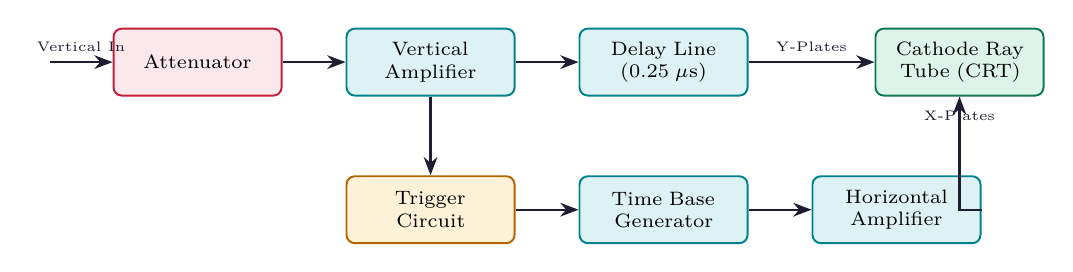
\begin{tikzpicture}[node distance=0.5cm and 0.8cm, thick, font=\small,
  sblock/.style={rectangle, draw=myteal, fill=hdrteal, text width=1.9cm,
    align=center, minimum height=0.85cm, font=\scriptsize, rounded corners=3pt, line width=0.7pt},
  sred/.style={rectangle, draw=myred, fill=hdrred, text width=1.9cm,
    align=center, minimum height=0.85cm, font=\scriptsize, rounded corners=3pt, line width=0.7pt},
  samber/.style={rectangle, draw=myamber, fill=hdramber, text width=1.9cm,
    align=center, minimum height=0.85cm, font=\scriptsize, rounded corners=3pt, line width=0.7pt},
  sgreen/.style={rectangle, draw=mygreen, fill=hdrgreen, text width=1.9cm,
    align=center, minimum height=0.85cm, font=\scriptsize, rounded corners=3pt, line width=0.7pt}]

  % Vertical Channel
  \node[sred] (att) {Attenuator};
  \node[sblock, right=of att] (vamp) {Vertical\\Amplifier};
  \node[sblock, right=of vamp] (delay) {Delay Line\\(0.25 $\mu$s)};
  
  % CRT Block
  \node[sgreen, right=1.6cm of delay] (crt) {Cathode Ray\\Tube (CRT)};

  % Horizontal Channel
  \node[samber, below=1.0cm of vamp] (trig) {Trigger\\Circuit};
  \node[sblock, right=of trig] (tb) {Time Base\\Generator};
  \node[sblock, right=of tb] (hamp) {Horizontal\\Amplifier};

  % Paths
  \draw[arrow] ($(att.west) - (0.8, 0)$) -- node[above, font=\tiny] {Vertical In} (att.west);
  \draw[arrow] (att) -- (vamp);
  \draw[arrow] (vamp) -- (delay);
  \draw[arrow] (delay) -- node[above, font=\tiny] {Y-Plates} (crt.west);
  
  \draw[arrow] (vamp.south) -- (trig.north);
  \draw[arrow] (trig) -- (tb);
  \draw[arrow] (tb) -- (hamp);
  \draw[arrow] (hamp) -| node[above, pos=0.85, font=\tiny] {X-Plates} (crt.south);
\end{tikzpicture}
\tcbset{breakable}
\end{tcolorbox}

\subsection{Key Functional Units}
\begin{itemize}[leftmargin=*, itemsep=3.5pt]
  \item \textbf{Cathode Ray Tube (CRT):} The heart of the CRO. Contains an electron gun (produces a focused electron beam), deflection plates (Y-plates for vertical input, X-plates for horizontal sweep), and a phosphor screen that glows when struck by electrons.
  \item \textbf{Delay Line:} Placed in the vertical channel. Since the trigger circuit and time-base generator require about $0.25\,\mu\text{s}$ to activate and generate the horizontal sweep, the vertical signal must be delayed by this duration. This ensures the sweep starts exactly when the signal begins, preventing the display from losing the leading edge.
  \item \textbf{Time Base Generator:} Generates a \textbf{saw-tooth ramp voltage} that sweeps the electron beam horizontally across the screen at a constant velocity, creating a linear time scale.
\end{itemize}

% ===============================================================================
\section{Lissajous Figures}
% ===============================================================================

When two sine waves are applied simultaneously to the horizontal and vertical deflection plates without the time base active, the resulting pattern on the screen is called a \textbf{Lissajous Figure}. It is used to measure phase difference and frequency.

\begin{tcolorbox}[formulabox, title={\textbf{Lissajous Wave Measurements}}]
\begin{enumerate}[leftmargin=*, itemsep=4.5pt, label=\arabic*.]
  \item \textbf{Phase Measurement ($\theta$):}
    For an ellipse centered at the origin, let $y_1$ be the y-intercept, and $y_2$ be the maximum vertical deflection:
    $$\sin \theta = \frac{y_1}{y_2} \implies \theta = \sin^{-1}\left(\frac{y_1}{y_2}\right)$$
    - If the major axis lies in Quadrants I \& III: $\theta$ is between $0^\circ$ and $90^\circ$ (or $270^\circ$--$360^\circ$).
    - If the major axis lies in Quadrants II \& IV: $\theta$ is between $90^\circ$ and $180^\circ$ (or $180^\circ$--$270^\circ$).
    - Circle $\implies \theta = 90^\circ$ or $270^\circ$. Straight line $\implies \theta = 0^\circ$ or $180^\circ$.
  \item \textbf{Frequency Measurement ($f_x, f_y$):}
    Let $N_h$ be the number of horizontal tangencies (intersections with a horizontal line at top), and $N_v$ be the number of vertical tangencies:
    $$\frac{f_y}{f_x} = \frac{N_h}{N_v} \implies f_y = f_x \cdot \frac{N_h}{N_v}$$
\end{enumerate}
\end{tcolorbox}

% ===============================================================================
\section{DSO \& Special Purpose Oscilloscopes}
% ===============================================================================

\subsection{Digital Storage Oscilloscope (DSO)}
A \textbf{DSO} digitizes, processes, and stores incoming signals in RAM before displaying them. 
- \textbf{Signal Flow:} Input signal $\to$ Attenuator $\to$ Sample \& Hold circuit $\to$ Analog-to-Digital Converter (ADC) $\to$ Digital memory (RAM) $\to$ Microprocessor $\to$ DAC / Display.
- \textbf{Advantages:} Permanent storage, pre-trigger viewing (displays signals before trigger event), mathematical processing (FFT, RMS, average), and easy data export.

\subsection{Dual Trace vs. Dual Beam CRO}
To display two channels on a screen:
\begin{itemize}[leftmargin=*, itemsep=3.5pt]
  \item \textbf{Dual Trace CRO:} Uses a single electron gun and single set of deflection plates. An electronic switch alternates rapidly between Channel A and B:
    - \textbf{Alternate Mode:} Displays one full sweep of Channel A, then one full sweep of Channel B. Best for high frequencies.
    - \textbf{Chop Mode:} Rapidly switches between A and B at a frequency of $\approx 100\,\text{kHz}$ during a single sweep. Best for low-frequency signals.
  \item \textbf{Dual Beam CRO:} Uses a special CRT with \textbf{two independent electron guns} and two sets of vertical deflection plates. Both signals are projected simultaneously. Extremely expensive but has no switching lag.
\end{itemize}

\newpage
% ===============================================================================
% MANDATORY QUICK REVISION PAGE
% ===============================================================================
\begin{center}
  {\large\bfseries\color{myred} Quick Revision --- Module 3}\\[3pt]
  {\small\color{mydark} Oscilloscopes (CRO \& DSO) $|$ OE-EC604A}
\end{center}
\noindent{\color{myred}\rule{\linewidth}{1.2pt}}
\vspace{4pt}

\begin{tcolorbox}[formulabox, title={\textbf{Key Oscilloscope Equations}}]
$$\text{Lissajous Phase Difference:} \quad \theta = \sin^{-1}\left(\frac{y_1}{y_2}\right)$$
$$\text{Frequency Calculation:} \quad \frac{f_y}{f_x} = \frac{N_{\text{tangencies\_horizontal}}}{N_{\text{tangencies\_vertical}}}$$
$$\text{CRO Probe Attenuation:} \quad v_{\text{in}} = v_{\text{scope}} \left(1 + \frac{R_{\text{probe}}}{R_{\text{scope}}}\right)$$
\end{tcolorbox}

\begin{tcolorbox}[defbox, title={\textbf{One-Line Definitions}}]
\begin{itemize}[leftmargin=*, itemsep=2.5pt, topsep=0pt]
  \item \textbf{Delay Line:} Coaxial cable delaying vertical signal to align with sweep startup trigger.
  \item \textbf{Time Base Circuit:} Generator producing saw-tooth sweep voltage to move beam linearly across horizontal axis.
  \item \textbf{Lissajous Pattern:} Figure generated on scope screen when two sine waves are fed to X and Y deflection plates.
  \item \textbf{Dual Trace:} Scope using single gun and electronic switch to show two signals on one screen.
  \item \textbf{DSO:} Digital Scope that samples incoming analog signals, converts them to digital data, and stores them in RAM.
  \item \textbf{10x Probe:} Passive attenuating probe containing a $9\,\text{M}\Omega$ resistor to increase input impedance to $10\,\text{M}\Omega$.
\end{itemize}
\end{tcolorbox}

\begin{tcolorbox}[exambox, title={\textbf{Frequently Asked / Viva Questions}}]
\begin{enumerate}[topsep=0pt, label=\textbf{Q\arabic*.}, itemsep=5pt]
  \item \Q{What is the primary purpose of the Delay Line in a CRO vertical channel?}
    The time base sweep generator requires around $0.25\,\mu\text{s}$ of processing delay to trigger after a signal arrives. If the vertical signal is fed directly to the Y-plates, it will reach the plates before the sweep starts, cutting off the leading edge of the waveform on the display. The delay line holds the vertical signal back by $0.25\,\mu\text{s}$ to synchronize it.
  \item \Q{Differentiate between Alternate Mode and Chop Mode in a Dual Trace CRO.}
    Alternate mode displays Channel A on one sweep and Channel B on the next sweep, which is suited for high-frequency signals. Chop mode switches back and forth between Channel A and B at a fast rate (e.g., $100\,\text{kHz}$) within a single sweep, making it suitable for low-frequency signals.
  \item \Q{Explain how phase difference is calculated from a Lissajous figure.}
    The phase difference is calculated using the formula $\theta = \sin^{-1}(y_1/y_2)$, where $y_1$ is the y-intercept (height where ellipse crosses vertical axis) and $y_2$ is the maximum vertical height of the ellipse.
  \item \Q{A Lissajous figure on screen has 3 horizontal tangencies and 2 vertical tangencies. The horizontal input frequency is $1\,\text{kHz}$. Calculate the vertical input frequency.}\\
    Using the tangency formula: $f_y / f_x = N_h / N_v \implies f_y / 1000 = 3 / 2$.\par
    $f_y = 1000 \times 1.5 = 1500\,\text{Hz} = 1.5\,\text{kHz}$.
  \item \Q{What are the advantages of a DSO over a conventional analog CRO?}
    A DSO can permanently store waveforms in memory, display pre-trigger signals (pre-trigger viewing), process signal data mathematically (FFT, peak detection, averaging), and export digital files directly to a computer.
  \item \Q{Explain the working of a 10x passive probe.}
    A 10x passive probe contains a $9\,\text{M}\Omega$ resistor in series with a shunt capacitor. When connected to a standard CRO channel (which has $1\,\text{M}\Omega$ input resistance), it forms a 10:1 voltage divider. This reduces the voltage reaching the scope to $1/10$th, but increases the overall input impedance to $10\,\text{M}\Omega$, minimizing circuit loading.
  \item \Q{What is the function of the phosphor coating on a CRT screen?}
    When high-energy electrons strike the phosphor coating, it fluoresces (emits visible light) and exhibits phosphorescence (continues to glow for a short duration), creating a stable trace of the electrical signal.
  \item \Q{Differentiate between Dual Trace and Dual Beam CROs.}
    Dual trace uses a single electron gun and single set of deflection plates, using switching circuits to alternate signals. Dual beam uses two independent electron guns and vertical deflection plates to project two beams simultaneously, eliminating switching lag.
  \item \Q{Explain the working of time base generator in a CRO.}
    It uses a UJT (uni-junction transistor) sweep circuit to charge a capacitor at a constant current rate, creating a linear rising ramp. Once it hits a peak, it discharges rapidly. This saw-tooth wave sweeps the beam horizontally.
  \item \Q{What is sampling in a Sampling Oscilloscope?}
    Sampling is a technique used to display extremely high-frequency signals (GHz range). The oscilloscope takes discrete amplitude samples at progressively delayed intervals over multiple successive cycles of the periodic signal, reconstructing the high-speed wave at a lower frequency.
\end{enumerate}
\end{tcolorbox}

\begin{tcolorbox}[tikzbox, title={Dual Trace vs Dual Beam Oscilloscope Comparison}]
\renewcommand{\arraystretch}{1.4}
\par\noindent
\begin{tabularx}{\linewidth}{|B{2.2cm}|>{\small\centering\arraybackslash}X|>{\small\centering\arraybackslash}X|}
\hline
\textbf{Feature} & \textbf{\color{myred}Dual Trace CRO} & \textbf{\color{myteal}Dual Beam CRO} \\
\hline
\textbf{Electron Gun} & Single electron gun. & Two independent electron guns. \\
\hline
\textbf{Deflection Plates} & Single set of vertical plates. & Two independent sets of vertical plates. \\
\hline
\textbf{Signal Display} & Time-shared switching (alt/chop). & Truly simultaneous display. \\
\hline
\textbf{Cost \& Design} & Moderate cost, simpler circuitry. & Extremely high cost, complex CRT tube. \\
\hline
\end{tabularx}
\end{tcolorbox}


% -- Module 4 -----------------------------------------------------------------
\modulestart{4}{Introduction \& Classification}

\section{Introduction \& Classification}
% ===============================================================================

A \textbf{Transducer} is a physical device that converts energy from one form into another, typically transforming a physical parameter (measurand) into a proportional electrical signal.

\subsection{Key Classifications}
\begin{itemize}[leftmargin=*, itemsep=3.5pt]
  \item \textbf{Active vs. Passive Transducers:}
    - \textbf{Active (Self-generating):} Generates its own electrical output without requiring an external power source (e.g., Piezoelectric crystal, Thermocouple, Solar cell).
    - \textbf{Passive:} Requires an external excitation voltage source to function, modulating its resistance, capacitance, or inductance (e.g., Strain gauge, LVDT, Thermistor, RTD).
  \item \textbf{Primary vs. Secondary Transducers:}
    - \textbf{Primary:} Interacts directly with the measurand, converting it to a mechanical displacement (e.g., Bourdon tube).
    - \textbf{Secondary:} Converts the output of the primary transducer into an electrical signal (e.g., LVDT connected to Bourdon tube).
  \item \textbf{Analog vs. Digital Transducers:}
    - \textbf{Analog:} Outputs a continuous amplitude voltage signal (e.g., Thermocouple).
    - \textbf{Digital:} Outputs discrete pulse trains or binary codes (e.g., Shaft encoder).
\end{itemize}

% ===============================================================================
\section{Strain Gauges \& Temperature Transducers}
% ===============================================================================

\subsection{Strain Gauges \& Gauge Factor Derivation}
A strain gauge measures mechanical strain based on the piezoresistive effect: when a wire is stretched, its resistance changes due to change in length, cross-sectional area, and resistivity.

\begin{tcolorbox}[formulabox, title={\textbf{Gauge Factor (G) Derivation}}]
Resistance of a wire is $R = \rho \cdot \frac{L}{A}$. Taking the natural log on both sides:
$$\ln R = \ln \rho + \ln L - \ln A$$
Differentiating with respect to strain $\epsilon$:
$$\frac{dR}{R} = \frac{d\rho}{\rho} + \frac{dL}{L} - \frac{dA}{A}$$
Since area $A = \frac{\pi D^2}{4} \implies \ln A = \ln(\pi/4) + 2\ln D \implies \frac{dA}{A} = 2\frac{dD}{D}$. Thus:
$$\frac{dR}{R} = \frac{dL}{L} - 2\frac{dD}{D} + \frac{d\rho}{\rho}$$
Poisson's ratio is defined as $\nu = -\frac{dD/D}{dL/L} \implies \frac{dD}{D} = -\nu \frac{dL}{L}$. Substituting this:
$$\frac{dR}{R} = \frac{dL}{L} + 2\nu\frac{dL}{L} + \frac{d\rho}{\rho} = \frac{dL}{L}(1 + 2\nu) + \frac{d\rho}{\rho}$$
Dividing both sides by longitudinal strain $\epsilon = dL/L$:
$$G = \frac{dR/R}{dL/L} = 1 + 2\nu + \frac{d\rho/\rho}{dL/L}$$
where:
- $1$: Resistance change due to length change.
- $2\nu$: Resistance change due to area change.
- $\frac{d\rho/\rho}{dL/L}$: Piezoresistive effect (resistivity change). For metals, $G \approx 2.0$.
\end{tcolorbox}

\subsection{Temperature Transducers}
\begin{itemize}[leftmargin=*, itemsep=3.5pt]
  \item \textbf{RTD (Resistance Temperature Detector):} Made of pure metals (Platinum/Nickel). Positive temperature coefficient (PTC) $\implies$ resistance increases linearly with temperature: $R_T = R_0(1 + \alpha T)$. Stable, highly accurate.
  \item \textbf{Thermistor:} Made of semiconductor oxides. High negative temperature coefficient (NTC) $\implies$ resistance decreases exponentially with temperature. Extremely sensitive but non-linear.
  \item \textbf{Thermocouple:} Active transducer based on the Seebeck effect: when two dissimilar metals are joined at two junctions held at different temperatures, an electromotive force (EMF) is generated ($E = aT + bT^2$). Self-powered, wide temperature range.
\end{itemize}

% ===============================================================================
\section{LVDT \& Other Special Transducers}
% ===============================================================================

\subsection{LVDT (Linear Variable Differential Transformer)}
An \textbf{LVDT} is a passive inductive transducer used to measure linear displacement.
- \textbf{Structure:} Consists of a single primary winding (excited by AC), two secondary windings ($S_1$ and $S_2$) wound symmetrically on a hollow cylinder, and a movable soft iron core inside.
- \textbf{Working:} Secondary windings are connected in \textbf{series opposition}, so the output voltage is $E_o = E_{s1} - E_{s2}$.
  - At \textbf{Null Position} (core exactly centered): Magnetic coupling to both secondaries is identical $\implies E_{s1} = E_{s2} \implies E_o = 0\,\text{V}$.
  - Displacement to \textbf{Left}: Coupling to $S_1$ increases $\implies E_{s1} > E_{s2} \implies E_o$ is in-phase with input.
  - Displacement to \textbf{Right}: Coupling to $S_2$ increases $\implies E_{s2} > E_{s1} \implies E_o$ is out-of-phase by $180^\circ$.

\begin{tcolorbox}[tikzbox, title={LVDT Circuit Diagram}]
\centering
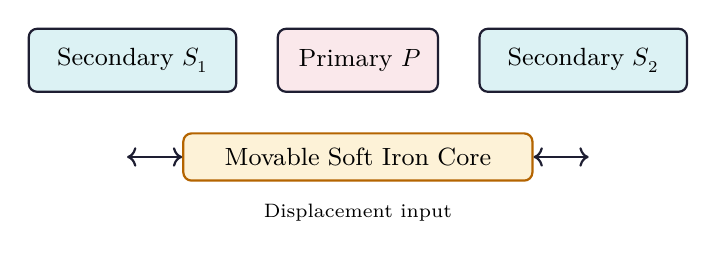
\begin{tikzpicture}[node distance=0.4cm and 0.5cm, thick, font=\small]
  % Define local node styles
  \tikzset{
    secblock/.style={rectangle, draw=mydark, fill=hdrteal, text width=2.4cm, align=center, minimum height=0.8cm, rounded corners=3pt},
    priblock/.style={rectangle, draw=mydark, fill=hdrred, text width=1.8cm, align=center, minimum height=0.8cm, rounded corners=3pt},
    coreblock/.style={rectangle, draw=myamber, fill=hdramber, text width=4.2cm, align=center, minimum height=0.6cm, rounded corners=3pt}
  }
  
  % Place Coils
  \node[secblock] (s1) {Secondary $S_1$};
  \node[priblock, right=of s1] (p) {Primary $P$};
  \node[secblock, right=of p] (s2) {Secondary $S_2$};
  
  % Place Core
  \node[coreblock, below=0.5cm of p] (core) {Movable Soft Iron Core};
  
  % Draw displacement arrows
  \draw[arrow, <->] ($(core.west) - (0.7, 0)$) -- (core.west);
  \draw[arrow, <->] (core.east) -- ($(core.east) + (0.7, 0)$);
  
  \node[below=0.15cm of core, font=\scriptsize] {Displacement input};
\end{tikzpicture}
\end{tcolorbox}

\subsection{Piezoelectric Transducer}
- \textbf{Principle:} Active transducer based on the piezoelectric effect. When mechanical force $F$ is applied to asymmetrical crystals (Quartz, Rochelle salt), electric charges $Q$ are generated on opposite faces: $Q = d \cdot F$, where $d$ is charge sensitivity. Output voltage is $V_o = g \cdot t \cdot P$ (where $g$ = voltage sensitivity, $t$ = thickness, $P$ = pressure).
- Used for dynamic force/pressure/vibration measurements. Cannot measure static displacement.

\newpage
% ===============================================================================
% MANDATORY QUICK REVISION PAGE
% ===============================================================================
\begin{center}
  {\large\bfseries\color{myred} Quick Revision --- Module 4}\\[3pt]
  {\small\color{mydark} Transducers $|$ OE-EC604A}
\end{center}
\noindent{\color{myred}\rule{\linewidth}{1.2pt}}
\vspace{4pt}

\begin{tcolorbox}[formulabox, title={\textbf{Key Transducer Formulas}}]
$$\text{Strain Gauge factor:} \quad G = 1 + 2\nu + \frac{d\rho/\rho}{d\epsilon} \qquad \frac{dR}{R} = G \cdot \epsilon$$
$$\text{RTD resistance:} \quad R_T = R_0(1 + \alpha T) \qquad \text{Thermocouple EMF:} \quad E = aT + bT^2$$
$$\text{Piezoelectric Voltage:} \quad V_o = g \cdot t \cdot P \qquad \text{where} \ g = \frac{d}{\epsilon_0 \cdot \epsilon_r}$$
\end{tcolorbox}

\begin{tcolorbox}[defbox, title={\textbf{One-Line Definitions}}]
\begin{itemize}[leftmargin=*, itemsep=2.5pt, topsep=0pt]
  \item \textbf{Transducer:} Device converting a non-electrical physical measurand into a proportional electrical signal.
  \item \textbf{Gauge Factor:} Ratio of fractional change in resistance to longitudinal strain in a strain gauge.
  \item \textbf{LVDT:} Linear Variable Differential Transformer; high-precision inductive linear displacement sensor.
  \item \textbf{Seebeck Effect:} Generation of an electric current/voltage at junction of two dissimilar metals due to thermal gradient.
  \item \textbf{Thermocouple:} Active thermal transducer measuring temperature based on Seebeck EMF.
  \item \textbf{RTD:} Positive temperature coefficient metal wire resistor used for linear temperature measurement.
  \item \textbf{Thermistor:} Highly sensitive, non-linear negative temperature coefficient semiconductor thermal sensor.
\end{itemize}
\end{tcolorbox}

\begin{tcolorbox}[exambox, title={\textbf{Frequently Asked / Viva Questions}}]
\begin{enumerate}[topsep=0pt, label=\textbf{Q\arabic*.}, itemsep=5pt]
  \item \Q{Differentiate between Active and Passive Transducers.}
    Active transducers are self-generating and do not require any external electrical source to produce output voltage (e.g., Piezoelectric sensor, Thermocouple). Passive transducers modify their electrical properties (resistance, inductance, capacitance) and require an external excitation source to function (e.g., Strain gauge, RTD, LVDT).
  \item \Q{Derive the expression for the Gauge Factor of a strain gauge.}
    The gauge factor is derived from wire resistance $R = \rho L / A$. Differentiating and dividing by longitudinal strain yields $G = 1 + 2\nu + \frac{d\rho/\rho}{dL/L}$, where $1$ represents change in length, $2\nu$ represents change in cross-sectional area, and the last term represents the piezoresistive effect.
  \item \Q{Explain the null position working of an LVDT.}
    In an LVDT, the primary coil is excited with AC, and the two secondaries are connected in series opposition ($E_o = E_{s1} - E_{s2}$). At the null position, the movable iron core is exactly centered, coupling equal magnetic flux to both secondaries. Therefore, $E_{s1} = E_{s2}$, resulting in a net output voltage of zero.
  \item \Q{A strain gauge has a gauge factor $G = 2.0$ and nominal resistance $R = 120\,\Omega$. Calculate the change in resistance when subjected to a strain of $1000\,\mu\text{strain}$.}\\
    Given: $G = 2.0$, $R = 120\,\Omega$, $\epsilon = 1000 \times 10^{-6} = 0.001$.\par
    $\Delta R = G \cdot \epsilon \cdot R = 2.0 \times 0.001 \times 120 = 0.24\,\Omega$.
  \item \Q{Compare RTD, Thermistor, and Thermocouple.}
    An RTD is a positive temp coefficient metallic sensor, highly linear and stable, but has low sensitivity. A thermistor is a negative temp coefficient semiconductor, extremely sensitive but highly non-linear. A thermocouple is an active self-powered bi-metal sensor with a very wide temp range but requires cold-junction compensation.
  \item \Q{Why can a piezoelectric transducer not measure static displacement/pressure?}
    A piezoelectric crystal generates electric charge when subjected to dynamic force. However, because the crystal has a finite leakage resistance and the connected display instrument has an input impedance, the generated charge leaks away quickly. Therefore, it is suited only for dynamic measurements (vibrations, impacts).
  \item \Q{What is the difference between primary and secondary transducers?}
    A primary transducer interacts directly with the physical parameter and converts it to a mechanical output (e.g., a Bourdon tube converting pressure to displacement). A secondary transducer converts this mechanical output into an electrical signal (e.g., an LVDT measuring the Bourdon tube displacement).
  \item \Q{What is the Seebeck effect and what are its applications?}
    The Seebeck effect is the generation of a small DC voltage when the junctions of two dissimilar metals are maintained at different temperatures. It forms the base working principle of thermocouples.
  \item \Q{Explain the difference between bounded and unbounded strain gauges.}
    Bounded strain gauges are cemented directly to the surface of the structure under test (e.g., beam) so they experience identical deformation. Unbounded strain gauges use fine wires stretched between fixed and movable frames, experiencing tension when the frame moves.
  \item \Q{What is magnetostriction and how is it used in transducers?}
    Magnetostriction is the property of ferromagnetic materials to undergo physical deformation (change length) when subjected to a magnetic field. It is used in magnetostrictive transducers to measure displacement or generate high-frequency ultrasonic waves.
\end{enumerate}
\end{tcolorbox}

\begin{tcolorbox}[tikzbox, title={Comparison of Temperature Transducers}]
\renewcommand{\arraystretch}{1.45}
\par\noindent
\begin{tabularx}{\linewidth}{|B{2.2cm}|Y|Y|Y|}
\hline
\textbf{Feature} & \textbf{\color{myred}RTD} & \textbf{\color{myteal}Thermistor} & \textbf{\color{myamber}Thermocouple} \\
\hline
\textbf{Working} & Resistance change in metals. & Resistance change in semiconductors. & EMF generation from bi-metal junction. \\
\hline
\textbf{Coefficient} & Positive (PTC). & Negative (NTC) / positive. & Not applicable. \\
\hline
\textbf{Linearity} & Excellent (Highly linear). & Non-linear (exponential). & Non-linear. \\
\hline
\textbf{Sensitivity} & Low. & Extremely High. & Low. \\
\hline
\textbf{Temp Range} & $-200^\circ\text{C}$ to $600^\circ\text{C}$ & $-100^\circ\text{C}$ to $300^\circ\text{C}$ & $-200^\circ\text{C}$ to $2000^\circ\text{C}$ \\
\hline
\end{tabularx}
\end{tcolorbox}


% -- Module 5 -----------------------------------------------------------------
\modulestart{5}{DC and AC Bridges}

\section{DC and AC Bridges}
% ===============================================================================

Bridges are comparison circuits used to measure resistance, inductance, capacitance, and impedance with high precision.

\subsection{Wheatstone Bridge}
The \textbf{Wheatstone Bridge} is a fundamental DC bridge used for measuring medium resistances ($1\,\Omega$ to $100\,\text{k}\Omega$).

\begin{tcolorbox}[defbox, title={\textbf{Wheatstone Bridge Principle}}]
It consists of four resistive arms forming a closed loop, with a DC source connected across one pair of opposite junctions and a null detector (galvanometer) across the other. When the potential difference across the galvanometer is zero, the bridge is balanced.
\end{tcolorbox}

\subsubsection{Derivation of Balance Equation}
Let the four resistive arms be $P$, $Q$, $R$, and $S$:
\begin{itemize}[leftmargin=*, itemsep=3pt]
  \item $P$ and $Q$ are fixed, known ratio arms.
  \item $R$ is the variable standard resistance.
  \item $S$ is the unknown resistance ($R_x$).
\end{itemize}
At balance, the current through the galvanometer is $I_g = 0$. This implies:
\begin{equation}
  V_B = V_D \implies I_1 P = I_2 R
\end{equation}
Since no current passes through the galvanometer, the current in arm $BC$ is $I_1$ and in arm $DC$ is $I_2$:
\begin{equation}
  I_1 = \frac{E}{P + Q} \qquad \text{and} \qquad I_2 = \frac{E}{R + S}
\end{equation}
Substituting these currents into the potential equation:
\begin{equation}
  \left(\frac{E}{P + Q}\right) P = \left(\frac{E}{R + S}\right) R \implies \frac{P}{P + Q} = \frac{R}{R + S}
\end{equation}
Cross-multiplying yields:
\begin{equation}
  P(R + S) = R(P + Q) \implies P R + P S = P R + Q R \implies P S = Q R \implies S = \frac{Q}{P} R
\end{equation}
Thus, the unknown resistance is:
\begin{equation}
  R_x = \frac{Q}{P} R
\end{equation}

\subsubsection{Limitations of Wheatstone Bridge}
It cannot measure low resistances ($< 1\,\Omega$) accurately because the contact resistances of terminals and the lead wire resistances are of similar magnitude, introducing significant errors.

\subsection{Kelvin Double Bridge}
The \textbf{Kelvin Double Bridge} is a modification of the Wheatstone bridge designed specifically to eliminate lead and contact resistances when measuring low resistances ($1\,\mu\Omega$ to $1\,\Omega$).

\begin{tcolorbox}[defbox, title={\textbf{Kelvin Double Bridge Concept}}]
It introduces a second set of ratio arms ($p$ and $q$) which are connected to a galvanometer to bypass the potential drop across the low-resistance connecting link ($r$) between the unknown low resistance ($R$) and standard low resistance ($S$).
\end{tcolorbox}

\subsubsection{Derivation of Balance Equation}
Let the main ratio arms be $P$ and $Q$, and the inner ratio arms be $p$ and $q$. The resistance of the connecting lead is $r$.
The galvanometer is connected between the junction of $P$ and $Q$ and the junction of $p$ and $q$. At balance, the potential difference across the galvanometer is zero.
The current $I$ divides at the connecting link:
\begin{itemize}[leftmargin=*, itemsep=3pt]
  \item Main branch current is $I$.
  \item The path through the inner ratio arms ($p+q$) is in parallel with the link resistance $r$.
\end{itemize}
The current through the link branch $p+q$ is:
\begin{equation}
  I_{pq} = I \cdot \frac{r}{p + q + r}
\end{equation}
The voltage drop across the branch $p$ is:
\begin{equation}
  V_p = I_{pq} \cdot p = I \left( \frac{p r}{p + q + r} \right)
\end{equation}
For balance, the ratio of potential drops across the primary arms must be equal:
\begin{equation}
  \frac{P}{Q} = \frac{R + V_p}{S + V_q} = \frac{R + I \left(\frac{p r}{p + q + r}\right)}{S + I \left(\frac{q r}{p + q + r}\right)}
\end{equation}
Cross-multiplying and solving for $R$:
\begin{equation}
  P \left[ S + \frac{q r}{p + q + r} \right] = Q \left[ R + \frac{p r}{p + q + r} \right]
\end{equation}
\begin{equation}
  P S + \frac{P q r}{p + q + r} = Q R + \frac{Q p r}{p + q + r}
\end{equation}
\begin{equation}
  Q R = P S + \frac{P q r - Q p r}{p + q + r}
\end{equation}
Dividing by $Q$:
\begin{equation}
  R = \frac{P}{Q} S + \frac{q r}{p + q + r} \left( \frac{P}{Q} - \frac{p}{q} \right)
\end{equation}
If we design the bridge such that the ratio of the inner arms equals the ratio of the outer arms:
\begin{equation}
  \frac{P}{Q} = \frac{p}{q}
\end{equation}
Then the term $\left(\frac{P}{Q} - \frac{p}{q}\right)$ becomes zero. The balance equation simplifies to:
\begin{equation}
  R = \frac{P}{Q} S
\end{equation}
Thus, the effect of the connecting lead resistance $r$ is completely eliminated.

\subsection{Maxwell Inductance-Capacitance Bridge}
The \textbf{Maxwell Bridge} is an AC bridge used to measure an unknown inductance by comparing it with a standard variable capacitor. It is suited for measuring medium-Q coils ($1 < Q < 10$).

\begin{tcolorbox}[tikzbox, title={Maxwell Inductance-Capacitance Bridge Circuit}]
\centering
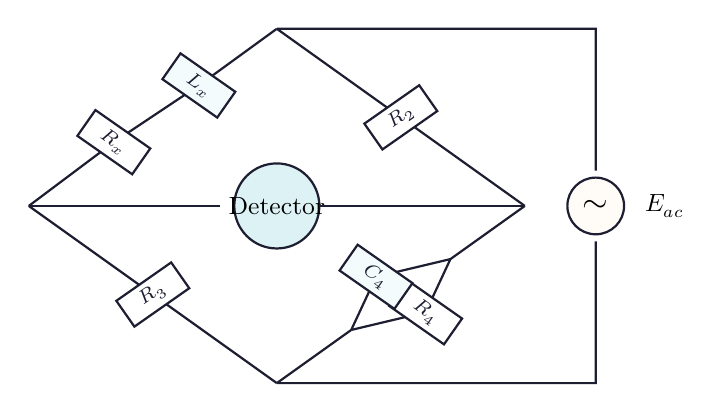
\begin{tikzpicture}[scale=0.9, thick, font=\small, >=Stealth]
  % Define main coordinates
  \coordinate (A) at (0, 2.5);
  \coordinate (B) at (-3.5, 0);
  \coordinate (C) at (0, -2.5);
  \coordinate (D) at (3.5, 0);

  % Draw Detector
  \draw[line] (B) -- (-0.8, 0);
  \draw[draw=mydark, fill=hdrteal] (0, 0) circle (0.6) node {Detector};
  \draw[line] (0.6, 0) -- (D);

  % Helper component node style
  \tikzset{
    comp/.style={rectangle, draw=mydark, fill=white, minimum width=0.85cm, minimum height=0.4cm, inner sep=2pt, font=\scriptsize}
  }

  % Arm AB (Top-Left): Rx and Lx in series
  \draw[line] (B) -- (-2.3, 0.9) node[comp, rotate=-35] (Rx) {$R_x$} -- (-1.1, 1.7) node[comp, fill=hdrteal!30, rotate=-35] (Lx) {$L_x$} -- (A);
  
  % Arm AD (Top-Right): R2
  \draw[line] (A) -- (1.75, 1.25) node[comp, rotate=35] (R2) {$R_2$} -- (D);

  % Arm BC (Bottom-Left): R3
  \draw[line] (B) -- (-1.75, -1.25) node[comp, rotate=35] (R3) {$R_3$} -- (C);

  % Arm DC (Bottom-Right): R4 in parallel with C4
  \coordinate (DCmid) at (1.75, -1.25);
  \draw[line] (D) -- (2.45, -0.75);
  % R4 branch
  \draw[line] (2.45, -0.75) -- (2.1, -1.5) node[comp, rotate=-35] (R4) {$R_4$} -- (1.05, -1.75);
  % C4 branch
  \draw[line] (2.45, -0.75) -- (1.4, -1.0) node[comp, fill=hdrteal!30, rotate=-35] (C4) {$C_4$} -- (1.05, -1.75);
  \draw[line] (1.05, -1.75) -- (C);

  % AC Source Loop
  \draw[line] (A) -- (4.5, 2.5) -- (4.5, 0.5);
  \draw[draw=mydark, fill=hdramber!20] (4.5, 0) circle (0.4) node {\large $\sim$};
  \draw[line] (4.5, -0.5) -- (4.5, -2.5) -- (C);
  \node[right=0.5cm of {4.5,0}, font=\small] {$E_{ac}$};
\end{tikzpicture}
\end{tcolorbox}

\subsubsection{Derivation of Balance Equation}
Let:
\begin{itemize}[leftmargin=*, itemsep=3pt]
  \item Arm 1 ($AB$): Impedance $Z_1 = R_x + j\omega L_x$ (unknown inductance and resistance).
  \item Arm 2 ($AD$): Impedance $Z_2 = R_2$ (non-inductive resistance).
  \item Arm 3 ($BC$): Impedance $Z_3 = R_3$ (non-inductive resistance).
  \item Arm 4 ($DC$): Impedance $Z_4$ consists of $R_4$ in parallel with $C_4$. Thus, its admittance $Y_4$ is:
    \begin{equation}
      Y_4 = \frac{1}{R_4} + j\omega C_4
    \end{equation}
\end{itemize}
The general AC bridge balance condition is:
\begin{equation}
  Z_1 \cdot Z_4 = Z_2 \cdot Z_3 \implies Z_1 = \frac{Z_2 Z_3}{Z_4} = Z_2 Z_3 Y_4
\end{equation}
Substitute the values of $Z_1$, $Z_2$, $Z_3$, and $Y_4$:
\begin{equation}
  R_x + j\omega L_x = R_2 R_3 \left( \frac{1}{R_4} + j\omega C_4 \right)
\end{equation}
\begin{equation}
  R_x + j\omega L_x = \frac{R_2 R_3}{R_4} + j\omega R_2 R_3 C_4
\end{equation}
Equating the real and imaginary parts on both sides:
\begin{equation}
  \text{Real Part:} \quad R_x = \frac{R_2 R_3}{R_4}
\end{equation}
\begin{equation}
  \text{Imaginary Part:} \quad L_x = R_2 R_3 C_4
\end{equation}
The Quality Factor ($Q$) of the inductor is:
\begin{equation}
  Q = \frac{\omega L_x}{R_x} = \frac{\omega (R_2 R_3 C_4)}{\left(\frac{R_2 R_3}{R_4}\right)} = \omega C_4 R_4
\end{equation}

\subsubsection{Advantages and Disadvantages}
\begin{itemize}[leftmargin=*, itemsep=3pt]
  \item \textbf{Advantages:} Balance equations are independent of frequency; simple relation for computing $L_x$ and $R_x$ separately.
  \item \textbf{Disadvantages:} Requires an expensive variable capacitor; not suitable for high-Q coils ($Q > 10$) because the required resistance $R_4$ becomes extremely high, making it impractical.
\end{itemize}

\newpage
% ===============================================================================
\section{Measurement of Non-Electrical Parameters}
% ===============================================================================

\subsection{Flow Measurement: Electromagnetic Flow Meter}
Electromagnetic flow meters measure the volumetric flow rate of an electrically conducting fluid.

\begin{tcolorbox}[defbox, title={\textbf{Working Principle (Faraday's Law)}}]
When a conductive fluid flows through a pipe of diameter $D$ across a transverse magnetic field of flux density $B$, an electromotive force (EMF) $E$ is induced across the electrodes perpendicular to the field:
\begin{equation}
  E = B \cdot D \cdot v
\end{equation}
where $v$ is the average fluid velocity.
\end{tcolorbox}

\subsubsection{Concept and Working}
\begin{itemize}[leftmargin=*, itemsep=3pt]
  \item A magnetic coil placed around the pipe creates a uniform magnetic field.
  \item As the conductive fluid (measurand) flows, it acts as a moving conductor, generating voltage.
  \item Metallic electrodes flush-mounted on the pipe walls pick up the induced voltage.
  \item The flow rate $Q$ is proportional to velocity: $Q = A \cdot v = \frac{\pi D^2}{4} \cdot \left(\frac{E}{B D}\right) = \frac{\pi D}{4 B} \cdot E \implies Q \propto E$.
\end{itemize}
- \textbf{Advantages:} Non-invasive (zero pressure drop), handles corrosive/slurry liquids, independent of viscosity, density, and temperature.
- \textbf{Disadvantages:} Fluid must be electrical-conducting ($> 5\,\mu\text{S/cm}$); cannot measure oil, gas, or pure water.

\subsection{Level Measurement}
\subsubsection{Capacitive Level Transducer}
Operates on the variation of capacitance between two concentric cylindrical electrodes placed in a vessel.
- \textbf{Non-Conducting Fluid:} Capacitance changes as the liquid level $h$ rises, displacing air:
  \begin{equation}
    C = \frac{2\pi\epsilon_0 [h\epsilon_r + (H - h)]}{\ln(b/a)}
  \end{equation}
  where $a$ and $b$ are the inner and outer electrode radii, $H$ is the total height, and $\epsilon_r$ is the liquid dielectric constant.
- \textbf{Conducting Fluid:} The probe is insulated with a thin dielectric material (e.g., Teflon). The fluid acts as the outer plate of the capacitor. The capacitance varies linearly with depth $h$.

\subsubsection{Ultrasonic Level Transducer}
Non-contact type sensor mounted at the top of the tank.
- \textbf{Working:} Emits ultrasonic pulses downward. The pulses reflect off the liquid surface and return to the transducer.
- \textbf{Formula:} The distance to the liquid surface $d$ is calculated from transit time $t$:
  \begin{equation}
    d = \frac{v \cdot t}{2} \qquad (\text{where } v = \text{velocity of sound in air})
  \end{equation}
  The liquid level is $h = H - d$, where $H$ is the total height of the tank.

\subsection{Pressure Measurement}
\subsubsection{LVDT-Based Pressure Cell}
A mechanical pressure-sensing element (bellows, diaphragm, or Bourdon tube) is used as the primary transducer to convert pressure into physical displacement. The core of an LVDT is connected to this element as the secondary transducer, converting displacement into an electrical output voltage.

\subsubsection{Pirani Vacuum Gauge}
A thermal conductivity gauge used to measure low pressures ($10^{-4}\,\text{torr}$ to $1\,\text{torr}$).
- \textbf{Working:} A heated tungsten filament is placed in a chamber connected to the vacuum system. As pressure decreases, the density of gas molecules decreases. Fewer molecules collide with the filament, reducing heat dissipation (thermal conductivity drops). The filament temperature increases, raising its electrical resistance. This resistance change is measured using a Wheatstone bridge.

\subsubsection{McLeod Vacuum Gauge}
An absolute calibration instrument used to measure very low pressures down to $10^{-6}\,\text{torr}$.
- \textbf{Working:} A gas sample of large initial volume $V$ at unknown low pressure $P$ is compressed into a small capillary tube of area $a$ to a much smaller volume. The compressed pressure is measured using a mercury column height difference $h$.
- \textbf{Formula:} Applying Boyle's Law ($P_1 V_1 = P_2 V_2$):
  \begin{equation}
    P \cdot V = (P + h) \cdot (a \cdot h)
  \end{equation}
  Since $P \ll h$ under compression, the unknown pressure is approximated as:
  \begin{equation}
    P \approx \frac{a \cdot h^2}{V}
  \end{equation}


\subsection{Humidity and Moisture Measurement}
Humidity indicates the water vapor content in the air, while moisture refers to the water content bound inside materials (e.g., soil, grains, wood).

\begin{tcolorbox}[defbox, title={\textbf{Relative Humidity (RH)}}]
Relative Humidity (RH) is the ratio of the actual water vapor pressure ($p_v$) to the saturation water vapor pressure ($p_s$) of air at the same temperature, expressed as a percentage:
\begin{equation}
  \text{RH} = \frac{p_v}{p_s} \times 100\%
\end{equation}
\end{tcolorbox}

\subsubsection{Sling Psychrometer (Wet/Dry Bulb Principle)}
A sling psychrometer is a classical instrument used to measure relative humidity by comparing dry-bulb and wet-bulb temperatures.
\begin{itemize}[leftmargin=*, itemsep=3.5pt]
  \item \textbf{Working Principle:} It consists of two identical thermometers mounted side-by-side:
    \begin{itemize}[leftmargin=*, itemsep=2.5pt, topsep=0pt]
      \item \textbf{Dry-Bul Thermometer ($T_d$):} Exposed directly to ambient air to measure standard dry air temperature.
      \item \textbf{Wet-Bul Thermometer ($T_w$):} Its bulb is covered with a clean cotton wick saturated with distilled water.
    \end{itemize}
  \item \textbf{Operation:} The user whirls/slings the psychrometer in the air. This rapid movement creates air flow, causing water to evaporate from the wet wick. Evaporation absorbs latent heat, cooling the wet bulb.
  \item \textbf{Humidity Determination:} The rate of evaporation (and thus cooling) depends on the moisture content in the air. 
    \begin{itemize}[leftmargin=*, itemsep=2.5pt, topsep=0pt]
      \item In dry air, evaporation is rapid, creating a large temperature difference ($T_d - T_w$, known as \textbf{psychrometric depression}).
      \item In fully saturated air (100\% RH), no evaporation occurs, and $T_d = T_w$.
    \end{itemize}
    Relative humidity is determined from psychrometric tables or charts using $T_d$ and the psychrometric depression ($T_d - T_w$).
\end{itemize}

\subsubsection{Electronic Hygrometers}
Electronic hygrometers are solid-state transducers that convert humidity into an electrical signal.
\begin{itemize}[leftmargin=*, itemsep=3.5pt]
  \item \textbf{Capacitive Hygrometer:}
    \begin{itemize}[leftmargin=*, itemsep=2.5pt, topsep=0pt]
      \item \textbf{Structure:} Consists of a thin hygroscopic polymer or metal-oxide dielectric layer placed between two metal electrodes. The top electrode is porous, allowing water vapor to pass through.
      \item \textbf{Working:} The polymer layer absorbs water vapor from air until equilibrium is reached. Since water has a high dielectric constant ($\epsilon_r \approx 80$) compared to the dry polymer dielectric ($\epsilon_r \approx 3$), water absorption increases the sensor capacitance:
        \begin{equation}
          C \approx C_0 (1 + \alpha \cdot \text{RH})
        \end{equation}
        where $C_0$ is dry capacitance and $\alpha$ is the humidity sensitivity coefficient.
    \end{itemize}
  \item \textbf{Resistive Hygrometer:}
    \begin{itemize}[leftmargin=*, itemsep=2.5pt, topsep=0pt]
      \item \textbf{Working:} Uses a hygroscopic salt (e.g., Lithium Chloride, LiCl) deposited on an insulating substrate between two electrodes. The salt absorbs moisture, generating mobile ions.
      \item \textbf{Resistance Change:} The electrical resistance decreases exponentially with increasing humidity.
    \end{itemize}
\end{itemize}

\begin{tcolorbox}[tikzbox, title={Structure of a Capacitive Humidity Sensor}]
\centering
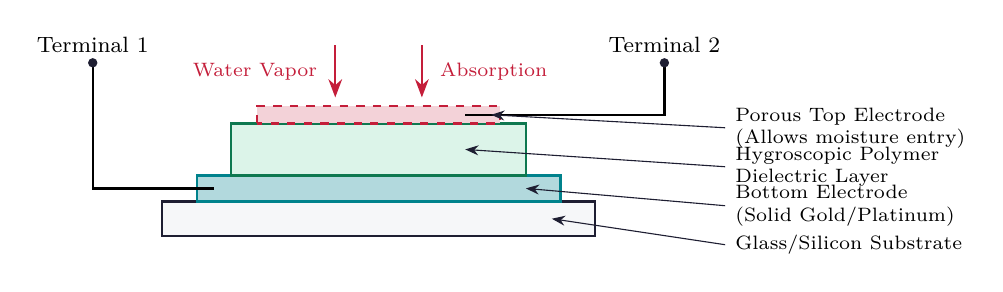
\begin{tikzpicture}[scale=1.1, thick, font=\small, >=Stealth]
  % Draw layers
  % Substrate (Glass/Silicon)
  \draw[fill=mygray, draw=mydark] (0, 0) rectangle (5, 0.4) coordinate (sub_mid);
  
  % Bottom Electrode (Solid Gold/Platinum)
  \draw[fill=myteal!30, draw=myteal] (0.4, 0.4) rectangle (4.6, 0.7) coordinate (bot_mid);
  
  % Dielectric Polymer Layer
  \draw[fill=hdrgreen, draw=mygreen] (0.8, 0.7) rectangle (4.2, 1.3) coordinate (poly_mid);
  
  % Top Electrode (Porous)
  \draw[fill=myred!20, draw=myred, dashed] (1.1, 1.3) rectangle (3.9, 1.5) coordinate (top_mid);

  % Terminals and contacts
  % Terminal 1 (Left - connected to Bottom Electrode)
  \draw (0.6, 0.55) -- (-0.8, 0.55) -- (-0.8, 2.0) node[circle, fill=mydark, inner sep=1.2pt] {} node[above] {\footnotesize Terminal 1};
  
  % Terminal 2 (Right - connected to Top Electrode)
  \draw (3.5, 1.4) -- (5.8, 1.4) -- (5.8, 2.0) node[circle, fill=mydark, inner sep=1.2pt] {} node[above] {\footnotesize Terminal 2};

  % Water Vapor / Absorption arrows
  \draw[redarrow] (2.0, 2.2) -- (2.0, 1.6) node[midway, left=0.1cm, font=\scriptsize\color{myred}] {Water Vapor};
  \draw[redarrow] (3.0, 2.2) -- (3.0, 1.6) node[midway, right=0.1cm, font=\scriptsize\color{myred}] {Absorption};

  % Callout Labels with leader lines (on the right/left)
  % We can place callouts on the right with a line pointing to each layer
  \node[anchor=west, align=left, font=\scriptsize] (lbl_top) at (6.5, 1.25) {Porous Top Electrode\\(Allows moisture entry)};
  \draw[->, thin, color=mydark] (lbl_top.west) -- (3.8, 1.4);

  \node[anchor=west, align=left, font=\scriptsize] (lbl_poly) at (6.5, 0.8) {Hygroscopic Polymer\\Dielectric Layer};
  \draw[->, thin, color=mydark] (lbl_poly.west) -- (3.5, 1.0);

  \node[anchor=west, align=left, font=\scriptsize] (lbl_bot) at (6.5, 0.35) {Bottom Electrode\\(Solid Gold/Platinum)};
  \draw[->, thin, color=mydark] (lbl_bot.west) -- (4.2, 0.55);

  \node[anchor=west, align=left, font=\scriptsize] (lbl_sub) at (6.5, -0.1) {Glass/Silicon Substrate};
  \draw[->, thin, color=mydark] (lbl_sub.west) -- (4.5, 0.2);
\end{tikzpicture}
\end{tcolorbox}

\subsubsection{Moisture Sensors}
Moisture measurement in materials (such as soil, paper, wood, or grain) is critical for industrial quality control and agriculture.
\begin{itemize}[leftmargin=*, itemsep=3.5pt]
  \item \textbf{Electrical Conductivity (Resistive) Method:}
    \begin{itemize}[leftmargin=*, itemsep=2.5pt, topsep=0pt]
      \item Operates by measuring electrical resistance between two metallic probes inserted into the material.
      \item Water is much more conductive than dry soil or organic fibers. Higher moisture content decreases resistance ($R \propto 1/\text{Moisture}$).
    \end{itemize}
  \item \textbf{Microwave Attenuation Method:}
    \begin{itemize}[leftmargin=*, itemsep=2.5pt, topsep=0pt]
      \item A microwave beam is transmitted through the material.
      \item Because water molecules have strong electric dipoles, they rotate rapidly in the microwave field, absorbing microwave energy.
      \item The attenuation (signal loss) and phase shift of the received signal are directly proportional to the total moisture content.
      \item This provides a non-contact, non-destructive, and continuous bulk measurement.
    \end{itemize}
\end{itemize}

\newpage
% ===============================================================================
\section{Data Acquisition Systems (DAS)}
% ===============================================================================

Data Acquisition Systems interface physical sensors with computers to measure and process parameters automatically.

\subsection{Analog and Digital DAS}
\begin{itemize}[leftmargin=*, itemsep=3.5pt]
  \item \textbf{Analog DAS:} Collects and displays data in continuous analog form (e.g., strip chart recorders, oscilloscope traces).
  \item \textbf{Digital DAS:} Converts analog signals into digital values for computer storage, display, and processing.
\end{itemize}

\begin{tcolorbox}[tikzbox, title={Digital Data Acquisition System Block Diagram}]
\centering
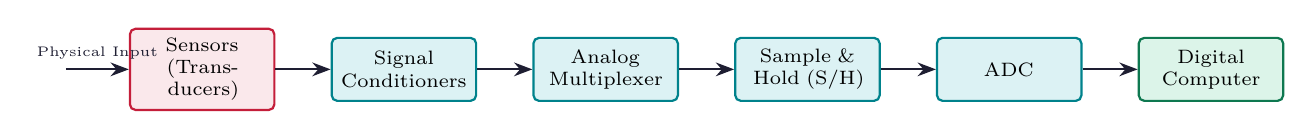
\begin{tikzpicture}[node distance=0.5cm and 0.8cm, thick, font=\scriptsize]
  \tikzset{
    sblock/.style={rectangle, draw=myteal, fill=hdrteal, text width=1.6cm, align=center, minimum height=0.8cm, rounded corners=2pt}
  }
  \node[sblock, fill=hdrred, draw=myred] (sensor) {Sensors\\(Transducers)};
  \node[sblock, right=0.7cm of sensor] (cond) {Signal\\Conditioners};
  \node[sblock, right=0.7cm of cond] (mux) {Analog\\Multiplexer};
  \node[sblock, right=0.7cm of mux] (sh) {Sample \&\\Hold (S/H)};
  \node[sblock, right=0.7cm of sh] (adc) {ADC};
  \node[sblock, right=0.7cm of adc, fill=hdrgreen, draw=mygreen] (pc) {Digital\\Computer};

  % Paths
  \draw[arrow] (sensor) -- (cond);
  \draw[arrow] (cond) -- (mux);
  \draw[arrow] (mux) -- (sh);
  \draw[arrow] (sh) -- (adc);
  \draw[arrow] (adc) -- (pc);
  
  % Input indicator
  \draw[arrow] ($(sensor.west) - (0.8, 0)$) -- node[above, font=\tiny] {Physical Input} (sensor.west);
\end{tikzpicture}
\end{tcolorbox}

\subsection{Roles of Key Digital DAS Components}
\begin{itemize}[leftmargin=*, itemsep=4pt]
  \item \textbf{Analog Multiplexer (MUX):} Sequences through multiple sensor channels, connecting one signal at a time to the common measurement chain. This avoids replicating expensive S/H and ADC components for every channel.
  \item \textbf{Sample and Hold (S/H) Circuit:} Captures the rapidly changing analog voltage at a specific instant and holds it constant at its output. This prevents errors during the time the ADC takes to perform a conversion.
  \item \textbf{ADC (Analog-to-Digital Converter):} Converts the held analog voltage into a proportional binary number (digital word) for the computer.
\end{itemize}

\newpage
% ===============================================================================
% MANDATORY QUICK REVISION PAGE
% ===============================================================================
\begin{center}
  {\large\bfseries\color{myred} Quick Revision --- Module 5}\\[3pt]
  {\small\color{mydark} Bridges, Parameter Measurement \& DAS $|$ OE-EC604A}
\end{center}
\noindent{\color{myred}\rule{\linewidth}{1.2pt}}
\vspace{4pt}

\begin{tcolorbox}[formulabox, title={\textbf{Key Module 5 Formulas}}]
\begin{align*}
  \text{Wheatstone Bridge:} \quad & R_x = \frac{Q}{P} R \qquad \text{Kelvin Double Bridge:} \quad R = \frac{P}{Q} S \ \left(\text{when} \ \frac{P}{Q} = \frac{p}{q}\right) \\
  \text{Maxwell } L_x: \quad & L_x = R_2 R_3 C_4 \qquad \text{Maxwell } R_x: \quad R_x = \frac{R_2 R_3}{R_4} \\
  \text{EM Flow EMF:} \quad & E = B \cdot D \cdot v \qquad \text{McLeod Vacuum:} \quad P \approx \frac{a \cdot h^2}{V} \\
  \text{Capacitive Humidity:} \quad & C \approx C_0 (1 + \alpha \cdot \text{RH}) \qquad \text{Relative Humidity:} \quad \text{RH} = \frac{p_v}{p_s} \times 100\%
\end{align*}
\end{tcolorbox}

\begin{tcolorbox}[defbox, title={\textbf{One-Line Definitions}}]
\begin{itemize}[leftmargin=*, itemsep=2.5pt, topsep=0pt]
  \item \textbf{Kelvin Double Bridge:} A bridge with double ratio arms to eliminate contact and lead resistance errors.
  \item \textbf{Maxwell Bridge:} An AC bridge used to measure medium-Q coil inductance using standard capacitance.
  \item \textbf{Electromagnetic Flow Meter:} An inductive flow meter measuring conductive fluid speed via Faraday's Law.
  \item \textbf{Pirani Gauge:} A thermal conductivity vacuum gauge measuring pressure via filament heat loss.
  \item \textbf{McLeod Gauge:} A mercury-filled vacuum gauge that compresses low-pressure gas to measure it hydrostatically.
  \item \textbf{Relative Humidity (RH):} Percent ratio of actual water vapor pressure to saturation vapor pressure.
  \item \textbf{Sling Psychrometer:} Instrument measuring humidity via dry-bulb and wet-bulb thermometers.
  \item \textbf{Hygrometer:} Electronic sensor designed to measure humidity in the atmosphere.
  \item \textbf{Multiplexer (MUX):} A switch routing multiple analog input channels sequentially to a single output line.
  \item \textbf{Sample and Hold (S/H):} A circuit holding analog voltage constant during the ADC conversion interval.
\end{itemize}
\end{tcolorbox}

\begin{tcolorbox}[exambox, title={\textbf{Frequently Asked / Viva Questions}}]
\begin{enumerate}[topsep=0pt, label=\textbf{Q\arabic*.}, itemsep=5pt]
  \item \Q{Why does a standard Wheatstone bridge fail to measure low resistances accurately?}
    At low resistances ($< 1\,\Omega$), the resistance of the connecting leads and contact terminals is significant relative to the test resistance. These lead resistances add directly to the measured resistance in a Wheatstone bridge, introducing massive measurement errors.
  \item \Q{Show how the lead resistance is eliminated in a Kelvin double bridge.}
    By incorporating inner ratio arms $p$ and $q$, the balance condition becomes $R = \frac{P}{Q} S + \frac{q r}{p + q + r}(\frac{P}{Q} - \frac{p}{q})$. Setting the outer ratios equal to the inner ratios ($\frac{P}{Q} = \frac{p}{q}$) cancels the second term, eliminating the lead link resistance $r$.
  \item \Q{Derive the balance equations for a Maxwell inductance-capacitance bridge.}
    Setting the opposite arm impedances equal, we get $Z_1 = Z_2 Z_3 Y_4$. Expanding: $R_x + j\omega L_x = R_2 R_3 (\frac{1}{R_4} + j\omega C_4)$. Separating real and imaginary parts yields $R_x = \frac{R_2 R_3}{R_4}$ and $L_x = R_2 R_3 C_4$.
  \item \Q{What are the limitations of a Maxwell bridge?}
    It is restricted to medium-Q coils ($1 < Q < 10$). For high-Q coils, $R_4$ must be extremely large, which is physically impractical. For low-Q coils ($Q < 1$), the balance converges very slowly due to sliding balance issues.
  \item \Q{An AC Maxwell bridge has $R_2 = 1\,\text{k}\Omega$, $R_3 = 2\,\text{k}\Omega$, $C_4 = 0.1\,\mu\text{F}$, and $R_4 = 100\,\text{k}\Omega$. Find the unknown $R_x$ and $L_x$.}\\
    Given: $R_x = \frac{R_2 R_3}{R_4} = \frac{10^3 \times (2 \times 10^3)}{100 \times 10^3} = 20\,\Omega$.\\
    $L_x = R_2 R_3 C_4 = 10^3 \times (2 \times 10^3) \times (0.1 \times 10^{-6}) = 0.2\,\text{H}$.
  \item \Q{Explain the working of an electromagnetic flow meter.}
    It operates on Faraday's Law ($E = B D v$). A magnetic field is applied across a pipe. The flowing conductive liquid acts as a conductor, generating an EMF across flush electrodes that is directly proportional to the average flow velocity.
  \item \Q{What is the principle of a Pirani vacuum gauge?}
    It works on the principle that the thermal conductivity of a gas is proportional to its pressure at low pressure. As chamber vacuum increases, less heat is conducted away from the filament, raising its temperature and resistance.
  \item \Q{Derive the pressure formula for a McLeod gauge.}
    Initial volume $V$ at pressure $P$ is compressed to volume $V_2 = a \cdot h$. The final pressure is $P + h$. By Boyle's Law: $P V = (P + h) a h = P a h + a h^2$. Since $P \ll h$, $P V \approx a h^2 \implies P \approx a h^2 / V$.
  \item \Q{Explain the dry-bulb and wet-bulb temperature principle of a Sling Psychrometer.}
    The dry bulb measures ambient temperature, while the wet bulb (covered in a wet wick) undergoes cooling due to water evaporation during slinging. The evaporation rate, and thus the wet-bulb temperature drop, is inversely proportional to relative humidity. In dry air, the drop is large; at 100\% humidity, the dry and wet bulb temperatures are equal ($T_d = T_w$).
  \item \Q{How does a capacitive humidity sensor detect relative humidity?}
    It uses a porous top electrode and a hygroscopic polymer dielectric. Water vapor penetrates the polymer. Since water has a high dielectric constant ($\epsilon_r \approx 80$) compared to the dry polymer ($\epsilon_r \approx 3$), the sensor capacitance increases proportionally to relative humidity.
  \item \Q{What is the principle of the microwave attenuation method for moisture measurement?}
    Water molecules have strong electrical dipoles that absorb microwave energy. When microwaves pass through a material, the signal attenuation and phase shift are directly proportional to the moisture content, providing a non-destructive bulk measurement.
  \item \Q{Why is a Sample and Hold circuit necessary before the ADC in digital DAS?}
    An ADC requires a finite time to convert an analog voltage into a digital word. If the analog input changes during this conversion period, the ADC output will suffer from aperture error. The S/H holds the input constant during conversion.
  \item \Q{Compare McLeod Gauge and Pirani Gauge.}
    McLeod gauge is an absolute, mechanical gauge working by volume compression, providing manual/discrete readings independent of gas type. Pirani gauge is a relative, thermal gauge providing continuous electrical output dependent on gas conductivity.
  \item \Q{What is the role of an analog multiplexer in a multi-channel DAS?}
    It acts as a rotary switch to connect multiple analog inputs sequentially to a single shared S/H and ADC. This reduces cost by eliminating the need for separate ADCs for each channel.
\end{enumerate}
\tcbset{colbacktitle=mypurple, coltitle=white}
\end{tcolorbox}

\begin{tcolorbox}[tikzbox, title={McLeod Gauge vs Pirani Gauge Comparison}]
\renewcommand{\arraystretch}{1.4}
\par\noindent
\begin{tabularx}{\linewidth}{|B{2.2cm}|Y|Y|}
\hline
\textbf{Feature} & \textbf{\color{myred}McLeod Gauge} & \textbf{\color{myteal}Pirani Gauge} \\
\hline
\textbf{Principle} & Gas volume compression (Boyle's Law). & Thermal conductivity variation. \\
\hline
\textbf{Reading Mode} & Discrete/Manual (batch process). & Continuous electrical reading. \\
\hline
\textbf{Gas Dependency} & Independent of gas composition. & Highly dependent on gas type. \\
\hline
\textbf{Output Signal} & Hydrostatic column level (height $h$). & Electrical resistance change. \\
\hline
\textbf{Calibration} & Absolute gauge (no calibration needed). & Relative gauge (needs calibration). \\
\hline
\textbf{Range} & $10^{-6}\,\text{torr}$ to $10^{-2}\,\text{torr}$ & $10^{-4}\,\text{torr}$ to $1\,\text{torr}$ \\
\hline
\end{tabularx}
\end{tcolorbox}


\end{document}
